\documentclass[aip,pof,reprint,superscriptaddress]{revtex4-2}

\usepackage{graphicx}
\usepackage{amsmath}
\usepackage{amssymb}
\usepackage{bm}
\usepackage{xcolor}
\usepackage{booktabs}
\usepackage{multirow}

\newcommand{\re}{\mathrm{Re}}

\begin{document}

\title{Physics-informed identification and independent numerical verification of conditional modal collapse in active control of lid-driven cavity flow}

\author{Ahmed Beniaiche}
\email{beniaiche\_ahmed25@yahoo.fr}
\affiliation{Laboratory of Fluid Mechanics, \'Ecole Militaire Polytechnique, Algiers, Algeria}

\date{\today}

\begin{abstract}
Identification of the actuation is formulated as a multi-objective optimization that combines the normalized mean-state dissipation and a prescribed target level of control energy. The problem is solved with a parametric physics-informed neural network (PINN) across a batch of Reynolds numbers in the range $100\le\re\le1000$, with distributed lid actuation for the lid-driven cavity. The identified control is then transferred to an independent lattice-Boltzmann solver for numerical verification under conditions deliberately chosen to differ from those of the identification, and its modal structure is examined by Fourier and Chebyshev projections of the realized control field. The identification recovers, across the tested actuation energies, network capacities, basis sizes, and aspect ratios, a branch dominated by a single stationary second spatial mode, which concentrates more than $91\%$ of the control energy at $\re=100$ and $500$. The independent solver reproduces this branch as a low-dissipation, quasi-stationary flow whose fluctuating kinetic energy remains below $1\%$ of the mean-flow kinetic energy. The branch is, however, not unique: a subset of random initializations reaches a time-dependent branch of comparable objective, modified-Chebyshev controls are temporally dominated and fail the adopted admissibility test, and the second-mode concentration weakens beyond $\re=1000$ and toward large actuation energies. We conclude that the second-mode-dominated control is a parameterization-conditioned, repeatedly recoverable branch of the identification problem rather than a universal optimum, and we emphasize the role of independent numerical verification and systematic branch analysis in discriminating such a branch from a parametrization-contingent alternative beyond the tested range.
\end{abstract}

\maketitle

\section{Introduction}\label{sec:intro}

\subsection{Active flow control and low-dimensional representations}

Active control of wall-bounded flows generally targets global quantities--drag, lift, or mixing--through distributed forcing at the boundaries, and reduced-order representations are commonly used to derive and interpret the resulting control laws \cite{brunton2015closed,gad2000flow,rowley2004model,noack2003hierarchy,taira2017modal}. The lid-driven cavity is a canonical testbed for such studies because its mean flow is well documented \cite{ghia1982high} and because its dominant large-scale features are energetically low-dimensional. However, the cavity also illustrates a difficulty that is common to several benchmark flows: the optimal forcing can be highly non-uniform, and its structure is not known in closed form. Consequently, the identification of distributed actuators is often performed numerically, either through adjoint-based approaches \cite{bewley2001dns,bergmann2005optimal} or, more recently, through deep-learning representations of the control law \cite{brunton2015closed,taira2017modal}.

\subsection{Physics-informed optimization and control identification}

Physics-informed neural networks (PINNs) embed the governing partial differential equations into the training loss through automatic differentiation \cite{raissi2019physics,karniadakis2021physics} and have been applied to forward and inverse problems in fluid mechanics \cite{raissi2020hidden,jin2021nsfnets,sun2020surrogate,cuomo2022,velivelli2024pinn}. In these formulations the network is trained to satisfy a physics-informed residual rather than a data loss, and the trained network provides a differentiable surrogate of the solution field over the entire domain. This property is attractive for control identification, because the control parameters can be optimized jointly with the approximate flow solution while the governing equations remain embedded in the objective. We adopt this approach for the lid-driven cavity, with a parametric network that approximates the steady two-dimensional incompressible flow and a separate coefficient network that represents the distributed lid actuation as a function of the Reynolds number.

\subsection{Structure and multiplicity in the control space}

A central question raised by optimization-based identification is whether the solution recovered by the optimization is unique. In inverse problems solved by gradient-based training, the solution is generally not unique in a strict sense: different random initializations can converge to different local minima, and the network capacity and parametrization of the control both influence the recovered branch. In the present work we treat this multiplicity explicitly and quantitatively. We characterize the identified control by its energy distribution over a Fourier basis, and we examine whether the dominant branch--a single stationary second spatial mode--survives systematic variation of the training seed, the actuation-energy target, the network capacity, the basis truncation, and the cavity aspect ratio. We then verify the recovered branch with an independent numerical method, a lattice-Boltzmann solver, that is deliberately different from the PINN approximation used during identification: it solves the transient problem, it uses a different discretization, and it is used without any physics-informed loss. Within this verification campaign, the Reynolds-number-dependent control identified by the PINN is applied as a prescribed boundary condition, including a reconstruction that retains only its dominant mode as an idealized test of the branch hypothesis.

\section{Problem formulation}\label{sec:problem}

\subsection{Governing equations}

We consider the steady, incompressible, two-dimensional lid-driven cavity on the rectangular domain $[0,L_x]\times[0,L_y]$, with the aspect ratio $\mathrm{AR}=L_x/L_y$. The flow is governed by the steady Navier--Stokes equations
\begin{equation}\label{eq:ns}
\re\,\bm u\cdot\nabla\bm u+\nabla p=\nabla^2\bm u,
\qquad\nabla\cdot\bm u=0,
\end{equation}
with the no-slip condition on the bottom and side walls,
\begin{equation}\label{eq:noslip}
u=0,\quad v=0\quad\text{on } y=0,\ x=0,\ x=L_x,
\end{equation}
and a prescribed horizontal velocity on the lid,
\begin{equation}\label{eq:lidbc}
u=\beta\,u_{\mathrm{lid}}(x),\quad v=0\quad\text{on } y=L_y.
\end{equation}
The control efficiency is measured by the normalized mean-state dissipation
\begin{equation}\label{eq:diss}
\varepsilon(\bm u)=\frac{\displaystyle\int_\Omega \omega^2\,\mathrm{d}\Omega}{\displaystyle\int_\Omega \omega_0^2\,\mathrm{d}\Omega},
\end{equation}
where $\omega=\partial_x v-\partial_y u$ is the vorticity, $\omega_0$ is the reference vorticity of the uncontrolled (uniform-lid) flow, and $\Omega=[0,L_x]\times[0,L_y]$. The Reynolds number is based on the reference lid velocity, $\re=\re_{\mathrm{ref}}$, and $\beta\in[0,1]$ scales the realized lid amplitude. The problem is parameterized by the Reynolds number $\re$ and by the target control energy $E^*$ introduced below.

\subsection{Physics-informed control formulation}

The actuation is a parametric function of the spatial coordinate along the lid and of the Reynolds number,
$u_{\mathrm{lid}}(x;\re)$, represented by a coefficient network as a linear combination of basis functions $\{\phi_{i,j}\}$,
see Section~\ref{sec:methods}. The control objective combines dissipation and a prescribed level of control energy. We write the identified lid control as
\begin{equation}\label{eq:energy}
E_{\mathrm{lid}}(\beta u_{\mathrm{lid}})=\frac{1}{L_xT}\int_0^T\int_0^{L_x} \bigl(\beta u_{\mathrm{lid}}(x,t)\bigr)^2\,\mathrm{d}x\,\mathrm{d}t,
\end{equation}
normalized so that the control-energy target $E^*$ is dimensionless. Because the parametrization is time-independent in the mean-state formulation of Section~\ref{sec:verification_campaign}, $E^*$ is effectively a target on the mean lid kinetic energy, and the realized value $E_r$ is measured from the trained control rather than imposed pointwise. In particular, a prescribed target level $E^*$ translates into a realization-dependent kinetic energy of the lid motion; its effect is examined separately through the actuation-energy sweep of Section~\ref{sec:energy}.

\begin{equation}\label{eq:targetenergy}
E^*=E_{\mathrm{lid}}^{0.25}\quad\text{(nominal working point)},
\end{equation}
with $E^*$ varied systematically in the sweep. At the nominal working point the identified control minimizes
\begin{equation}\label{eq:multiobj}
\mathcal{J}(\bm u,\beta,u_{\mathrm{lid}};\re)=\varepsilon(\bm u)+\alpha\,E_{\mathrm{lid}}(\beta u_{\mathrm{lid}}),
\end{equation}
where $\alpha$ weights the control-energy penalty. The physical-mechanism hypothesis embedded in this formulation is that the mean state can be softened toward lower dissipation by a suitable distribution of the lid forcing.

\section{Methods}\label{sec:methods}

\subsection{Parametric physics-informed neural network}

The velocity and pressure fields are represented by a fully connected neural network $\bm u_{\bm\theta}(x,y)$, $p_{\bm\theta}(x,y)$ with two hidden layers of 64 neurons each, an activated output for velocity, and a trainable output for pressure, following the standard PINN construction \cite{raissi2019physics,karniadakis2021physics}. The Reynolds number is an additional input, scaled as $R=\re/\re_{\mathrm{max}}$. The control is represented by a separate coefficient network that maps $R$ to the coefficients of the chosen basis (Section~\ref{sec:fourier}), so that the lid velocity is
\begin{equation}\label{eq:ctrlnet}
u_{\mathrm{lid}}(x;\re)=\sum_{i,j}c_{i,j}(\re)\,\phi_{i,j}(x),
\end{equation}
where the basis functions $\phi_{i,j}$ are the Fourier modes used in the parametrization. Spatial derivatives are computed by automatic differentiation.

\subsection{Fourier representation of the distributed control}\label{sec:fourier}

The control is expanded in a joint spatio-temporal Fourier basis
\begin{equation}\label{eq:phi}
\phi_{i,j}(x,t)=\sin\!\Bigl((i+1)\pi\frac{x}{L_x}\Bigr)\cos\!\Bigl(j\pi\frac{t}{T}\Bigr),
\qquad i,j\ge0,
\end{equation}
on the windowed interval $t\in[0,T]$ with $T=1$, which is also the window used for the LBM verification in Section~\ref{sec:verification_campaign}. The spatial variable is implicitly scaled onto $[0,1]$, and modal indices are counted from zero: the first spatial mode is $\sin(\pi x/L_x)$, the second is $\sin(2\pi x/L_x)$, and so on. In the baseline parametrization the network is trained with $n_{mx}=6$ spatial and $n_{mt}=5$ temporal modes. A modified-Chebyshev parametrization with the same number of modes and the same normalization is trained in parallel to test the basis dependence of the identified control; it is used only to assess the robustness of the branch, not to claim optimality. The smoothness of the identified control is controlled by the decay of the modal coefficients, and the realized control energy is measured on the full representation.

\subsection{Modal projection and control-energy decomposition}

Let $U=u_{\mathrm{lid}}(x,t)$ denote the realized (trained, continuous-in-time) control field on the $200\times200$ space--time grid used for post-processing. The projection of $U$ onto the mode $\phi_{i,j}$ is
\begin{equation}\label{eq:projection}
a_{i,j}=\frac{\displaystyle\sum_{n,m}W_{n,m}\,U_{n,m}\,\phi_{i,j}(x_n,t_m)}{\displaystyle\sum_{n,m}W_{n,m}\,\phi_{i,j}^2(x_n,t_m)},
\end{equation}
where the weights $W_{n,m}$ are the 2D trapezoidal quadrature weights (unit grid spacing with half-weight edges). The modal energy is
\begin{equation}\label{eq:modalenergy}
E_{i,j}=a_{i,j}^2\sum_{n,m}W_{n,m}\,\phi_{i,j}^2(x_n,t_m)\Big/\Delta,
\end{equation}
with area $\Delta=L_xT$, and the total represented energy is
\begin{equation}\label{eq:totalmodalenergy}
E_{\mathrm{tot}}=\frac{1}{\Delta}\sum_{n,m}W_{n,m}\,U_{n,m}^2.
\end{equation}
The second-mode fraction and the temporal fraction are then
\begin{equation}\label{eq:f2}
f_2=\frac{E_{1,0}}{E_{\mathrm{tot}}},\qquad
f_t=\frac{\displaystyle\sum_{j>0}E_{i,j}}{E_{\mathrm{tot}}}.
\end{equation}
The word \emph{modal collapse} is used in this article to denote the concentration of the control energy into a single stationary spatial mode (mode $(2,0)$ in the physical indexing used throughout, i.e.\ $i=1,\,j=0$ in the zero-based indexing of the basis), quantified by the fraction $f_2$. The label \emph{conditional} emphasizes that this collapse is observed for the tested settings (parametrization, targets, seeds, capacities), not claimed to be universal. Importantly, the temporal basis functions $\cos(j\pi t)$ remain mutually orthogonal on the interval $[0,1]$:
\begin{equation}\label{eq:ortho}
\int_0^1\cos(j\pi t)\cos(k\pi t)\,\mathrm{d}t=0\qquad(j\ne k),
\end{equation}
so the retained modal energies provide an additive decomposition of the represented control field, up to the numerical accuracy of the quadrature and projection.

\subsection{Physics-informed multi-objective loss}

The training loss combines the residual loss $\mathcal{L}_{\mathrm{pde}}$, the boundary loss $\mathcal{L}_{\mathrm{bc}}$, the dissipation objective $\mathcal{L}_{\mathrm{diss}}$, the control-energy penalty $\mathcal{L}_{\mathrm{ctrl}}$, and a variance regularization $\mathcal{L}_{\mathrm{var}}$:
\begin{equation}\label{eq:loss}
\mathcal{L}=\mathcal{L}_{\mathrm{pde}}+\mathcal{L}_{\mathrm{bc}}+\mathcal{L}_{\mathrm{diss}}+\mathcal{L}_{\mathrm{ctrl}}+\mathcal{L}_{\mathrm{var}},
\end{equation}
with
\begin{equation}\label{eq:lpde}
\mathcal{L}_{\mathrm{pde}}=\frac{1}{N_p}\sum_{n}\Bigl\|\re\,\bm u\cdot\nabla\bm u+\nabla p-\nabla^2\bm u\Bigr\|^2+\Bigl\|\nabla\cdot\bm u\Bigr\|^2,
\end{equation}
\begin{equation}\label{eq:lbc}
\mathcal{L}_{\mathrm{bc}}=\frac{1}{N_b}\sum_{n}\Bigl\|\bm u-\bm u_{\mathrm{bc}}\Bigr\|^2_{\partial\Omega_n},
\end{equation}
\begin{equation}\label{eq:ldiss}
\mathcal{L}_{\mathrm{diss}}=\varepsilon(\bm u),
\end{equation}
\begin{equation}\label{eq:lctrl}
\mathcal{L}_{\mathrm{ctrl}}=\alpha\,\bigl(E_{\mathrm{lid}}-E^*\bigr)^2,
\end{equation}
\begin{equation}\label{eq:lvar}
\mathcal{L}_{\mathrm{var}}=\lambda\,\operatorname{Var}\bigl(u_{\mathrm{lid}}\bigr),
\end{equation}
where $N_p$, $N_b$ are the numbers of collocation and boundary points, and $\alpha$, $\lambda$ are weights. The dissipation is evaluated on a uniform grid via the finite-difference vorticity field. The variance term penalizes the spread of the control profile along the lid, so that smooth, low-energy controls are preferred; its influence on branch selection is investigated explicitly through the loss-ablation study of Section~\ref{sec:ablation}. Training uses the Adam optimizer \cite{kingma2015adam} with a learning-rate schedule and a fixed seed for reproducibility; the random-initialization dependence is analyzed in the seed campaign of Section~\ref{sec:robustness_seeds}.

\subsection{Training procedure}

The models are trained with the architecture above for $10^5$ epochs at a learning rate of $10^{-3}$, with early stopping monitored on the PDE residual. The Reynolds number is swept in a batch: a set of Reynolds values is sampled uniformly in $[100,1000]$ and the parametric network is trained once for all of them. The control coefficients are the output of the coefficient network at the input Reynolds number, and the mean-state solution is evaluated at the corresponding $\re$. The nominal working point is $L_x=L_y=1$ (square cavity), $E^*=0.25$, seed 42, for the analyses of Sections~\ref{sec:baseline}--\ref{sec:verification_campaign}.

\section{Systematic robustness and branch analysis}\label{sec:robustness}

The robustness of the identified branch is characterized by repeating the identification under systematic perturbations of the training and problem settings. For each setting, the modal structure of the realized control is extracted with the projection of Section~\ref{sec:fourier}, and the branch is labeled by its dominant spatial--temporal mode. Throughout, the realized control energy $E_r$ is the one that results from training, not the target $E^*$.

\subsection{Training stochasticity and branch sensitivity}\label{sec:robustness_seeds}

Ten independent training runs are performed at $\re=500$, $E^*=0.25$, with seeds $0,\dots,9$ and the nominal architecture. For each run, the branch and the modal fractions are recorded (Table~\ref{tab:seeds} in Section~\ref{sec:seeds}). The runs are grouped by their branch label: a \emph{spatial branch} dominated by the stationary second mode ($f_2\ge86\%$), a \emph{temporal branch} dominated by the first time-dependent mode ($f_t\ge97\%$), or an \emph{intermediate} partition.

\subsection{Loss-term ablation and reweighting}\label{sec:ablation-methods}

The influence of each loss term is isolated by reweighting it, or removing it, one at a time at the nominal settings. The full loss is compared with the residual-only loss, with the dissipation removed, and with the variance term removed or strongly weighted. The switching between the branches under these reweightings is reported in Table~\ref{tab:ablation} (Section~\ref{sec:ablation}).

\subsection{Network-capacity robustness}\label{sec:arch}

The hidden-layer width is varied between 16 and 128 and the depth between two and four layers, at the nominal settings, seed 42. The number of parameters and the modal fractions of the realized control are recorded; a branch is considered robust if the dominant mode and the concentration level persist across the tested capacities.

\subsection{Control-space truncation}\label{sec:modecount}

The spatial and temporal resolutions of the basis are varied: $n_{mx}\times n_{mt}\in\{4\times3,6\times1,6\times3,6\times5,8\times5,8\times9\}$. For each truncation the realized control is retrained and its modal content is recorded (Table~\ref{tab:archmode} in Section~\ref{sec:archmode}).

\subsection{Actuation-energy dependence}\label{sec:energy-methods}

The control-energy target is varied through $E^*=0.01,0.05,0.10,0.25,0.50,1.00,2.00$ at $\re=500$, seed 42, and the realized energy, modal fractions, and spatial structure are recorded (Table~\ref{tab:energy} in Section~\ref{sec:energy}).

\subsection{Aspect-ratio sensitivity}\label{sec:ar-methods}

The domain is elongated to $\mathrm{AR}=2{:}1$ ($L_x=2$, $L_y=1$) with the same physical setup, and the identification is repeated at the nominal settings. The realized lid profiles are compared with the square-cavity ones, and the branch is re-examined (Table~\ref{tab:ar} in Section~\ref{sec:ar}).

\subsection{Control-parametrization dependence}\label{sec:param-methods}

The control is also identified under an alternative parametrization with the same capacity and training settings: a modified-Chebyshev basis. The realized controls of the two bases are then compared at $\re=100,500,1000$ in the independent LBM solver (Table~\ref{tab:param} in Section~\ref{sec:param}).

\subsection{Independent numerical verification campaign}\label{sec:verification_campaign}

The identified controls (complete PINN control and its dominant-mode truncation) are transferred to an independent lattice-Boltzmann solver for the LBM verification, at the operating conditions fixed by the identified control itself, i.e.\ the realized energy $E_r$ is applied and no re-optimization is performed. The verification protocols cover: (i) the LBM solver benchmark against the reference data of Ghia \emph{et al.}~\cite{ghia1982high}; (ii) the grid-convergence analysis of the dissipation metric; (iii) the realized flows under the four lid profiles; (iv) the time-dependent assessment of the Fourier and Chebyshev branches, in which the fluctuating kinetic energy is compared with the mean-flow kinetic energy on the LBM time horizon. The fluctuation diagnostics are computed from the time-resolved LBM solution $u(t),v(t)$ as the temporal average over the window $t\in[0,1]$ of the kinetic energy of the deviation from the windowed mean,
\begin{equation}\label{eq:kfluct}
K_{\mathrm{fluct}}=\frac{1}{2}\Bigl\langle \|u-\bar u\|_2^2+\|v-\bar v\|_2^2\Bigr\rangle,
\end{equation}
and the mean-flow kinetic energy as
\begin{equation}\label{eq:kmean}
K_{\mathrm{mean}}=\frac{1}{2}\Bigl\langle \|\bar u\|_2^2+\|\bar v\|_2^2\Bigr\rangle,
\end{equation}
where the angle brackets denote the windowed temporal average. The resulting fluctuating-to-mean-flow kinetic-energy ratio
\begin{equation}\label{eq:rk}
R_K=\frac{K_{\mathrm{fluct}}}{K_{\mathrm{mean}}}
\end{equation}
is used as the operational metric of quasi-stationarity defined in Sec.~\ref{sec:lbm}. The control is considered admissible if $R_K<1\%$ over the window.

\section{LBM verification methodology}\label{sec:lbm}

\subsection{Independent lattice-Boltzmann solver}

The verification solver is a two-dimensional lattice-Boltzmann code with the MRT collision operator \cite{succi2001lattice}, $\tau$-dependent transport coefficients, and a standard Bhatnagar--Gross--Krook forcing term. The cavity is discretized with $N=256$ points per dimension at the production resolution; the grid-convergence behavior is established in Section~\ref{sec:gci}. The Reynolds number is imposed through the relaxation parameter and the Mach number is kept below $0.1$. The solver is validated against the reference steady data of Ghia \emph{et al.}~\cite{ghia1982high} at $\re=100$ and $\re=1000$; the velocity profiles on the centerlines are compared in Section~\ref{sec:ghia}. The time horizon $T=1$ (in viscous units) is fixed by the advection time scale and is used for both the steady diagnostics (realized flows) and the time-dependent diagnostics (fluctuations).

The lid boundary condition is imposed with a velocity-profile reconstruction that matches the PINN representation at the grid points:
\begin{equation}\label{eq:lbm_lid}
u(x,L_y;t)=\hat u_{\mathrm{lid}}(x),\qquad \hat u_{\mathrm{lid}}(x)=u_{\mathrm{lid}}(x;\re)\Big|_{\mathrm{PINN}},
\end{equation}
i.e.\ the trained control is interpolated onto the LBM grid and applied as a Dirichlet condition, with the realized amplitude, for the duration of the window. The second-mode idealized control used in the grid-convergence and profile studies is the pure harmonic $A_2\sin(2\pi x/L_x)$ whose amplitude matches the second-mode projection of the PINN control.

\subsection{Admissible steady diagnostics}

The realized steady flows are diagnosed with two dissipation-based metrics. First, the integrated dissipation of the realized flow relative to the uniform-lid reference,
\begin{equation}\label{eq:lbm_diss}
\varepsilon_{\mathrm{LBM}}=\frac{\displaystyle\int_\Omega \omega^2\,\mathrm{d}\Omega}{\displaystyle\int_\Omega \omega_{\mathrm{uniform}}^2\,\mathrm{d}\Omega},
\end{equation}
measured with the same quadrature as in the definition of $\varepsilon$ (Eq.~\eqref{eq:diss}). Second, the second-mode response of the mean vertical centerline velocity,\\
$u(0.5,y)$, projected onto $\sin(2\pi y/L_y)$:
\begin{equation}\label{eq:lbm_phi}
a_2^{\mathrm{flow}}=\frac{\displaystyle\sum_{n}W_n\,u(0.5,y_n)\sin\!\Bigl(\pi\frac{y_n}{L_y}\Bigr)}{\displaystyle\sum_{n}W_n\sin^2\!\Bigl(\pi\frac{y_n}{L_y}\Bigr)},
\end{equation}
the one-dimensional quadrature weight $W_n$ being the trapezoidal weight. This quantity is compared with the control coefficient $a_2^{\mathrm{ctrl}}$ of the PINN representation. The Reynolds-number dependence of both metrics is reported in Section~\ref{sec:redep} (Fig.~\ref{fig:reyn}).

\subsection{Operational quasi-stationarity criterion}\label{sec:stationarity}

For controls that vary in time, the realized flow is not, in general, steady, and stationarity itself becomes an output of the verification rather than an assumption. We assess quasi-stationarity operationally: a control branch is called quasi-stationary if the fluctuating kinetic energy of the realized time-dependent solution remains below $1\%$ of the mean-flow kinetic energy over the window, i.e.\ $R_K<K^*=1\%$ (Eq.~\eqref{eq:rk}). This criterion is deliberately conservative: it does not assert exact stationarity, but it guarantees that the steady diagnostics of Sections~\ref{sec:dissipation}--\ref{sec:ghia} are representative. The criterion is applied to the Fourier and Chebyshev branches in Sections~\ref{sec:fourier_admis} and \ref{sec:cheb_lbm}.

\subsection{PINN-to-LBM transfer protocol}

The transfer from the PINN model to the LBM solver is a three-step, one-directional procedure. First, the trained coefficient network is evaluated at the input Reynolds number and the control profile is reconstructed on the LBM grid. Second, the realized amplitude is measured from the trained control and imposed as a boundary condition in the solver. Third, the solver is run on the window, and the diagnostics of Section~\ref{sec:stationarity} are computed without any feedback to the PINN. This procedure separates the identification and verification stages:
\[
\boxed{\;\text{identification (PINN, physics-informed loss)}\quad\longrightarrow\quad
\text{verification (LBM, transient solver, no PINN loss)}\;}
\]
no exchange of gradients, residuals, or parameters occurs between the two stages within the verification campaign.

\section{Results}\label{sec:results}

\subsection{Baseline Fourier branch}\label{sec:baseline}

The identification at the nominal settings ($\re=500$, $E^*=0.25$, seed 42) recovers a control whose dominant mode is the stationary second spatial harmonic. The resulting modal structure is summarized in Table~\ref{tab:baseline} and Fig.~\ref{fig:modal}.

\begin{figure}[t]
\centering
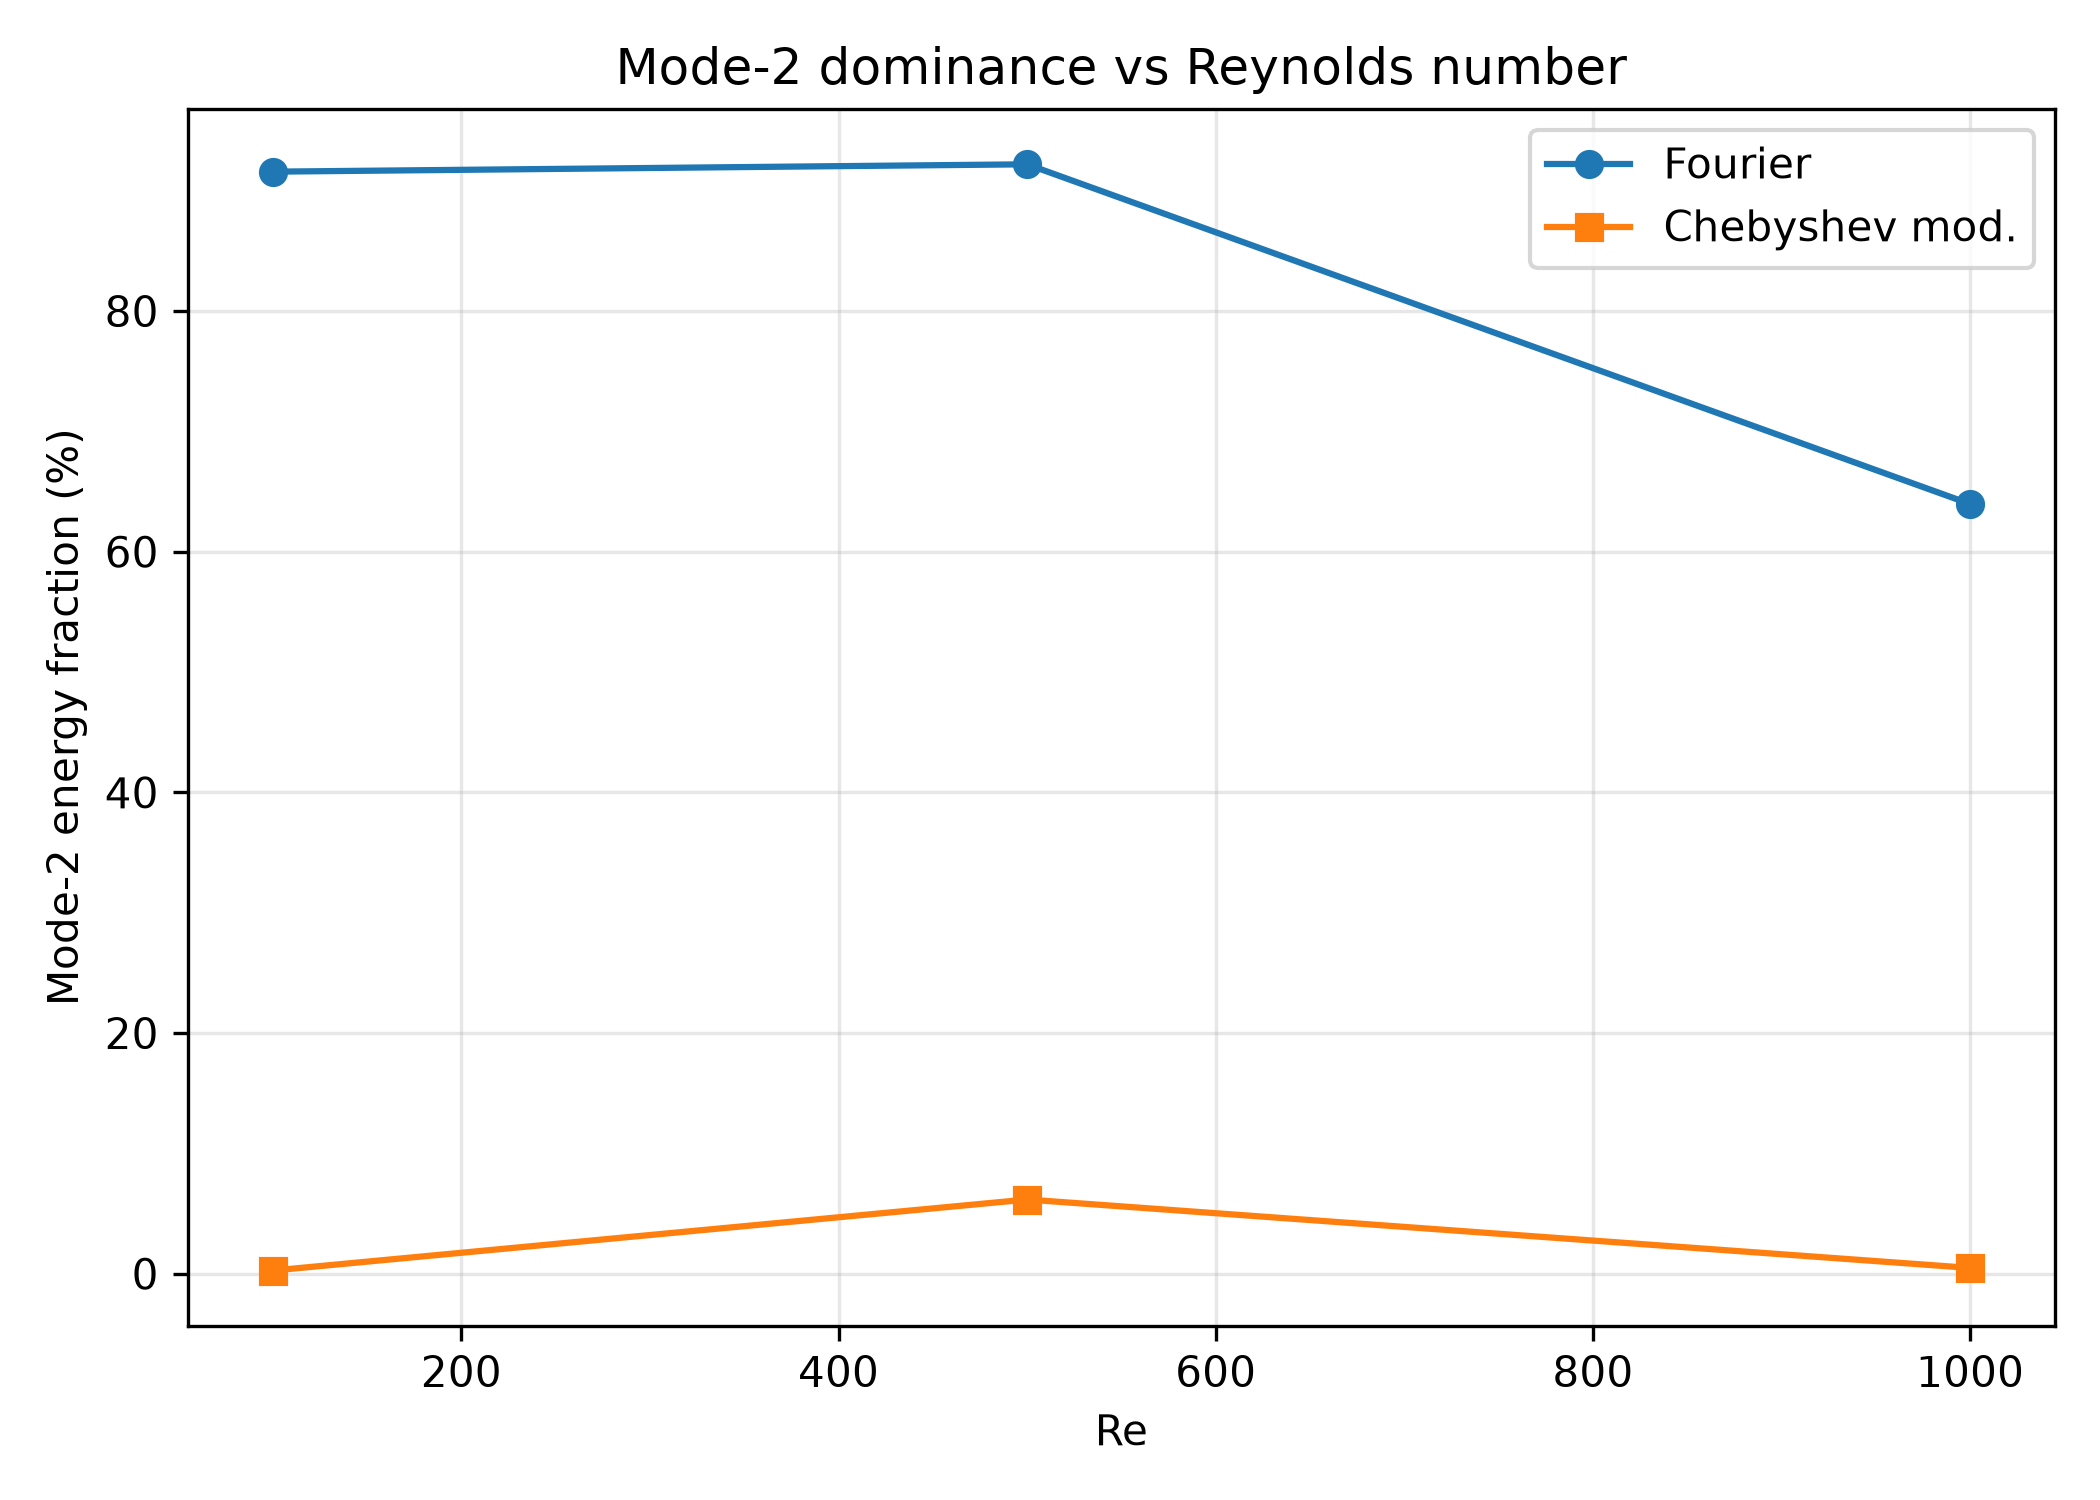
\includegraphics[width=0.49\linewidth]{figures/fig1_modal_fractions.png}\hfill
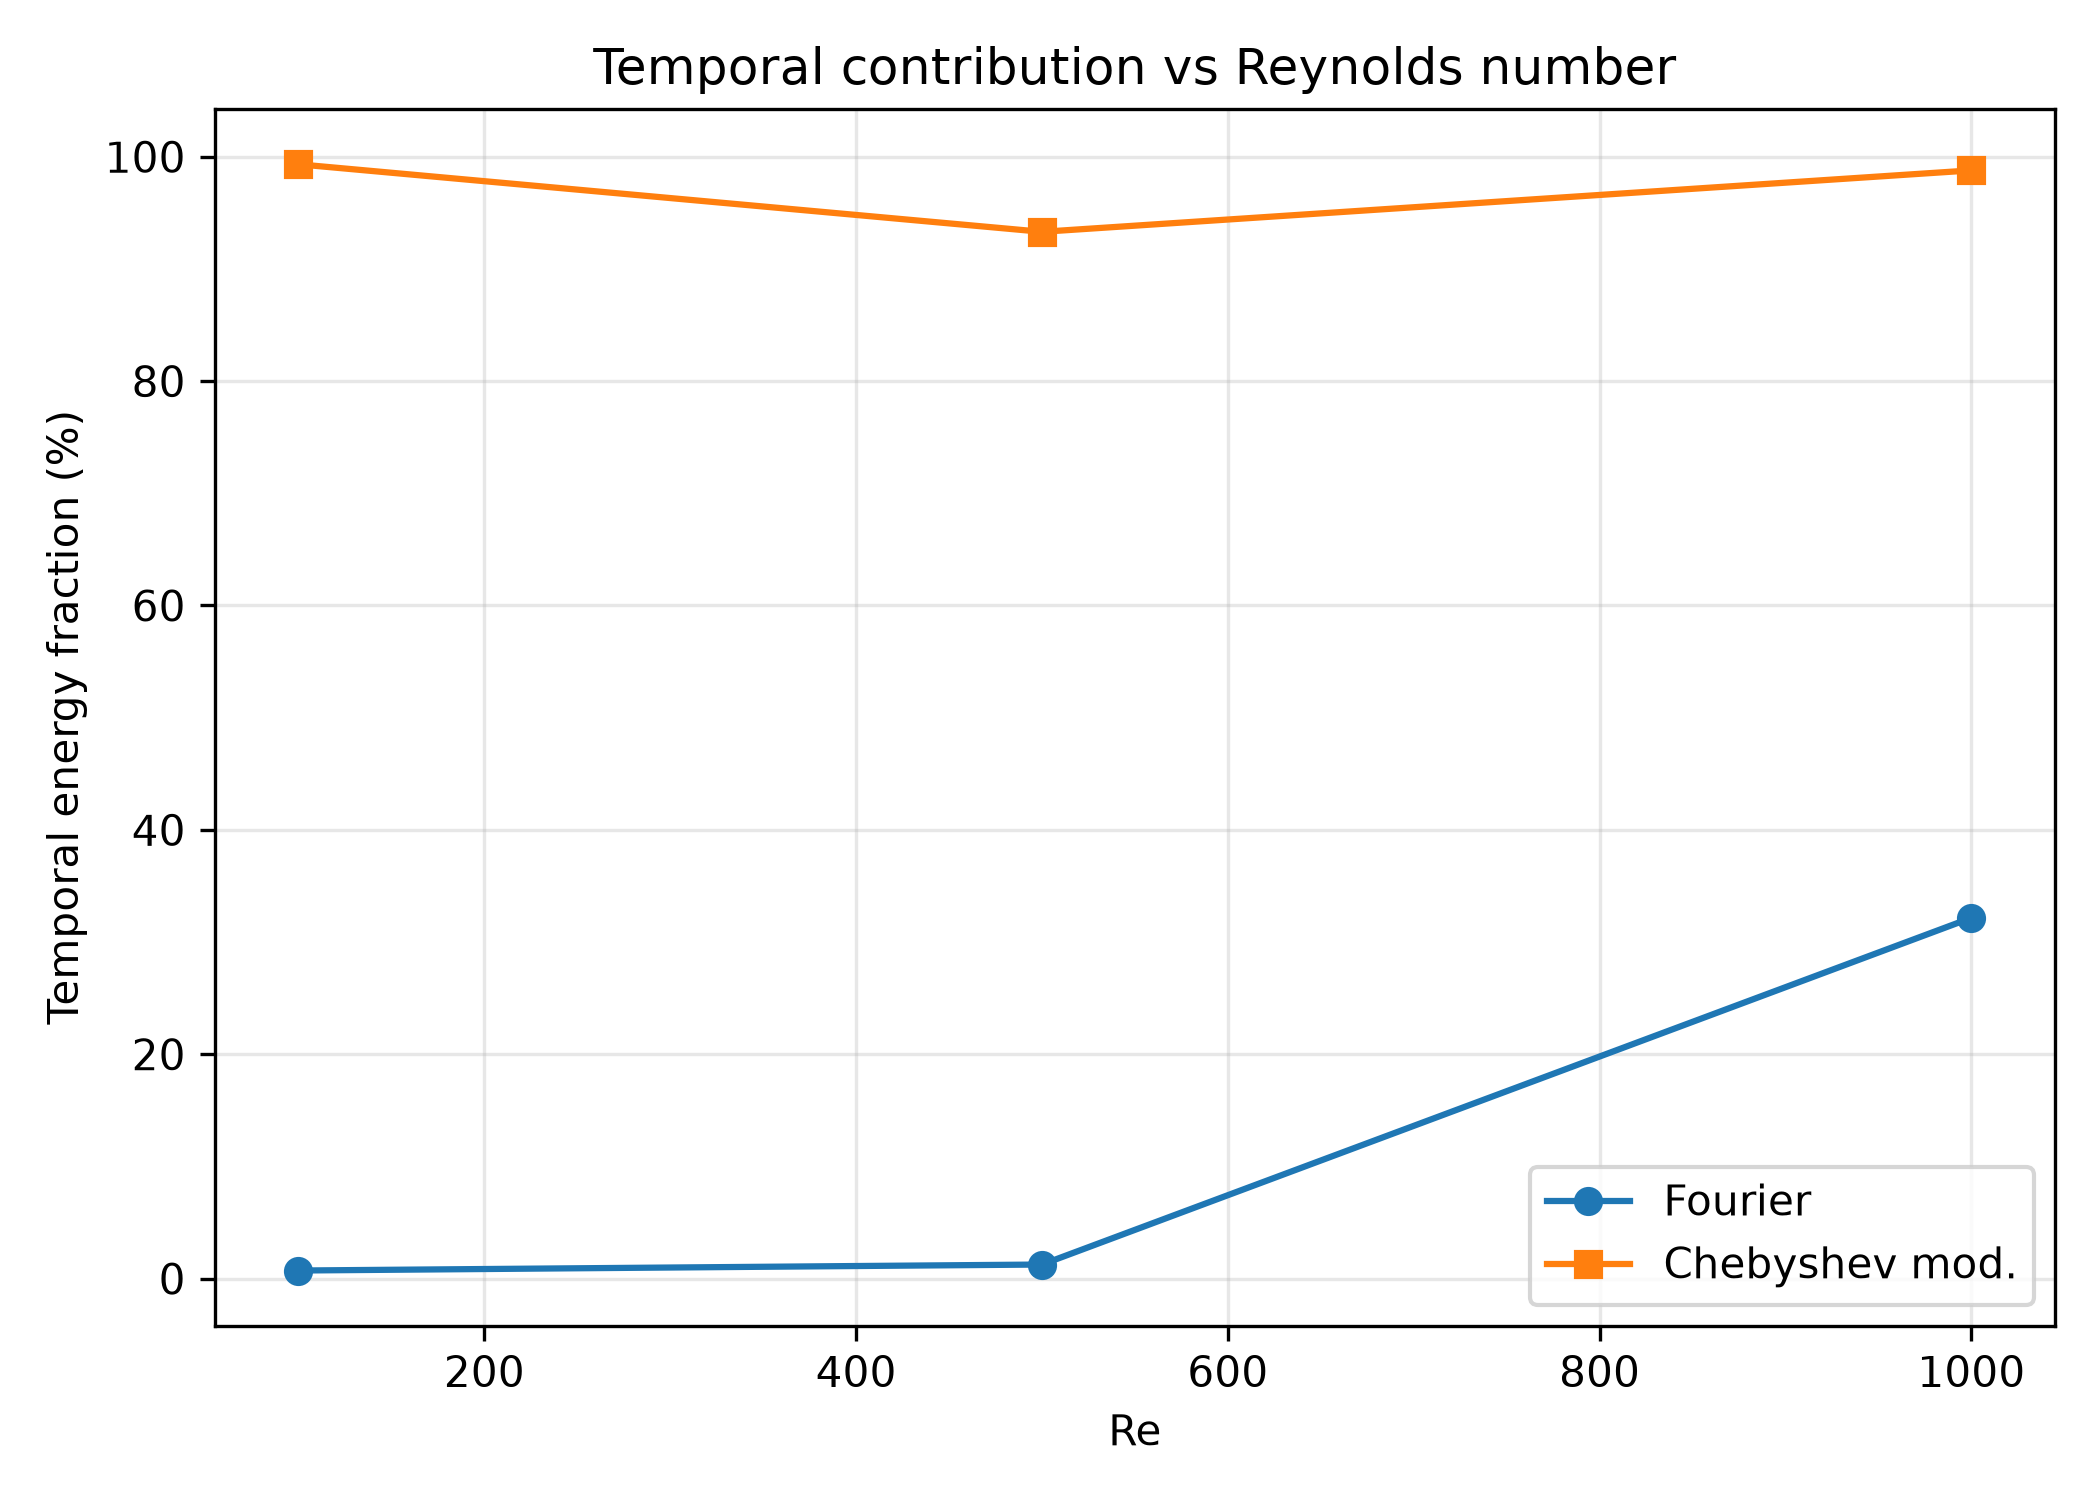
\includegraphics[width=0.49\linewidth]{figures/fig2_temporal_fractions.png}
\caption{\label{fig:modal} Second-mode energy fraction $f_2$ (left) and temporal energy fraction $f_t$ (right) of the identified control as functions of the Reynolds number, for the Fourier basis (circles) and the modified-Chebyshev basis (squares). The Fourier branch concentrates more than $91\%$ of the control energy in the stationary second spatial mode at $\re=100$ and $500$; at $\re=1000$ the second mode remains the largest contribution but its share drops to $64\%$ while the temporal content grows to $32\%$, delimiting the range over which the modal concentration is strong. The Chebyshev branch is temporally dominated at every Reynolds number.}
\end{figure}

\begin{table}[t]
\caption{\label{tab:baseline} Baseline modal content of the identified controls ($E^*=0.25$, seed 42): realized energy $E_r$, second-mode fraction $f_2$, temporal fraction $f_t$, and second-mode coefficient $A_2$, for the Fourier and modified-Chebyshev parametrizations.}
\centering
\begin{tabular}{lccc}
\toprule
Parametrization & $E_r$ & $f_2$ (\%) & $f_t$ (\%) \\
\midrule
Fourier, $\re=100$ & 0.2581 & 91.6 & 0.7 \\
Fourier, $\re=500$ & 0.2534 & 92.2 & 1.2 \\
Fourier, $\re=1000$ & 0.2687 & 64.0 & 32.2 \\
\midrule
Chebyshev, $\re=100$ & 0.2890 & 0.3 & 99.3 \\
Chebyshev, $\re=500$ & 0.2850 & 6.2 & 93.3 \\
Chebyshev, $\re=1000$ & 0.2908 & 0.5 & 98.8 \\
\bottomrule
\end{tabular}
\end{table}

The Fourier branch is characterized by the concentration of the control energy into a single stationary mode, with $A_2=0.6876$ at $\re=100$ and $A_2=0.6835$ at $\re=500$ (Table~\ref{tab:param}); the remaining energy is distributed over subdominant stationary and time-dependent modes. The Chebyshev control is qualitatively different: its realized energy is spread over time-dependent modes and its second-mode fraction is negligible. This contrasting behavior is the basis of the branch comparison of Sections~\ref{sec:param} and \ref{sec:cheb_lbm}.

\subsection{Reynolds-number dependence}\label{sec:redep}

The branch persists for $100\le\re\le800$ and degrades between $\re=800$ and $\re=1000$: the second-mode fraction remains above $91\%$ up to $\re=800$ and drops to $64\%$ at $\re=1000$ (Fig.~\ref{fig:modal}). The transition is accompanied by a growth of the temporal content from $1.2\%$ to $32.2\%$ (Table~\ref{tab:baseline}). The Reynolds-number dependence of the realized flow is consistent with this structural change: the second-mode response of the mean field and the total enstrophy of the realized flows retain their low-dissipation character at every Reynolds number, with a mild degradation toward $\re=1000$. Concretely, the centerline amplitude $a_2^{\mathrm{flow}}$ of the realized mean flow is positive and small in magnitude ($\sim3\times10^{-3}$, $6\times10^{-3}$, and $5\times10^{-2}$ at $\re=100$, $500$, and $1000$), and the enstrophy of the controlled branch lies markedly below that of the uniform lid at every Reynolds number (Fig.~\ref{fig:reyn}). As a state quantity extracted from the realized flow, $a_2^{\mathrm{flow}}$ is distinct from the control coefficient $a_2^{\mathrm{ctrl}}$ (labeled $A_2$ in the tables): the two quantities track each other in trend, but not in magnitude, the centerline response remaining one to two orders of magnitude below the control coefficient.

\begin{figure}[!t]
\centering
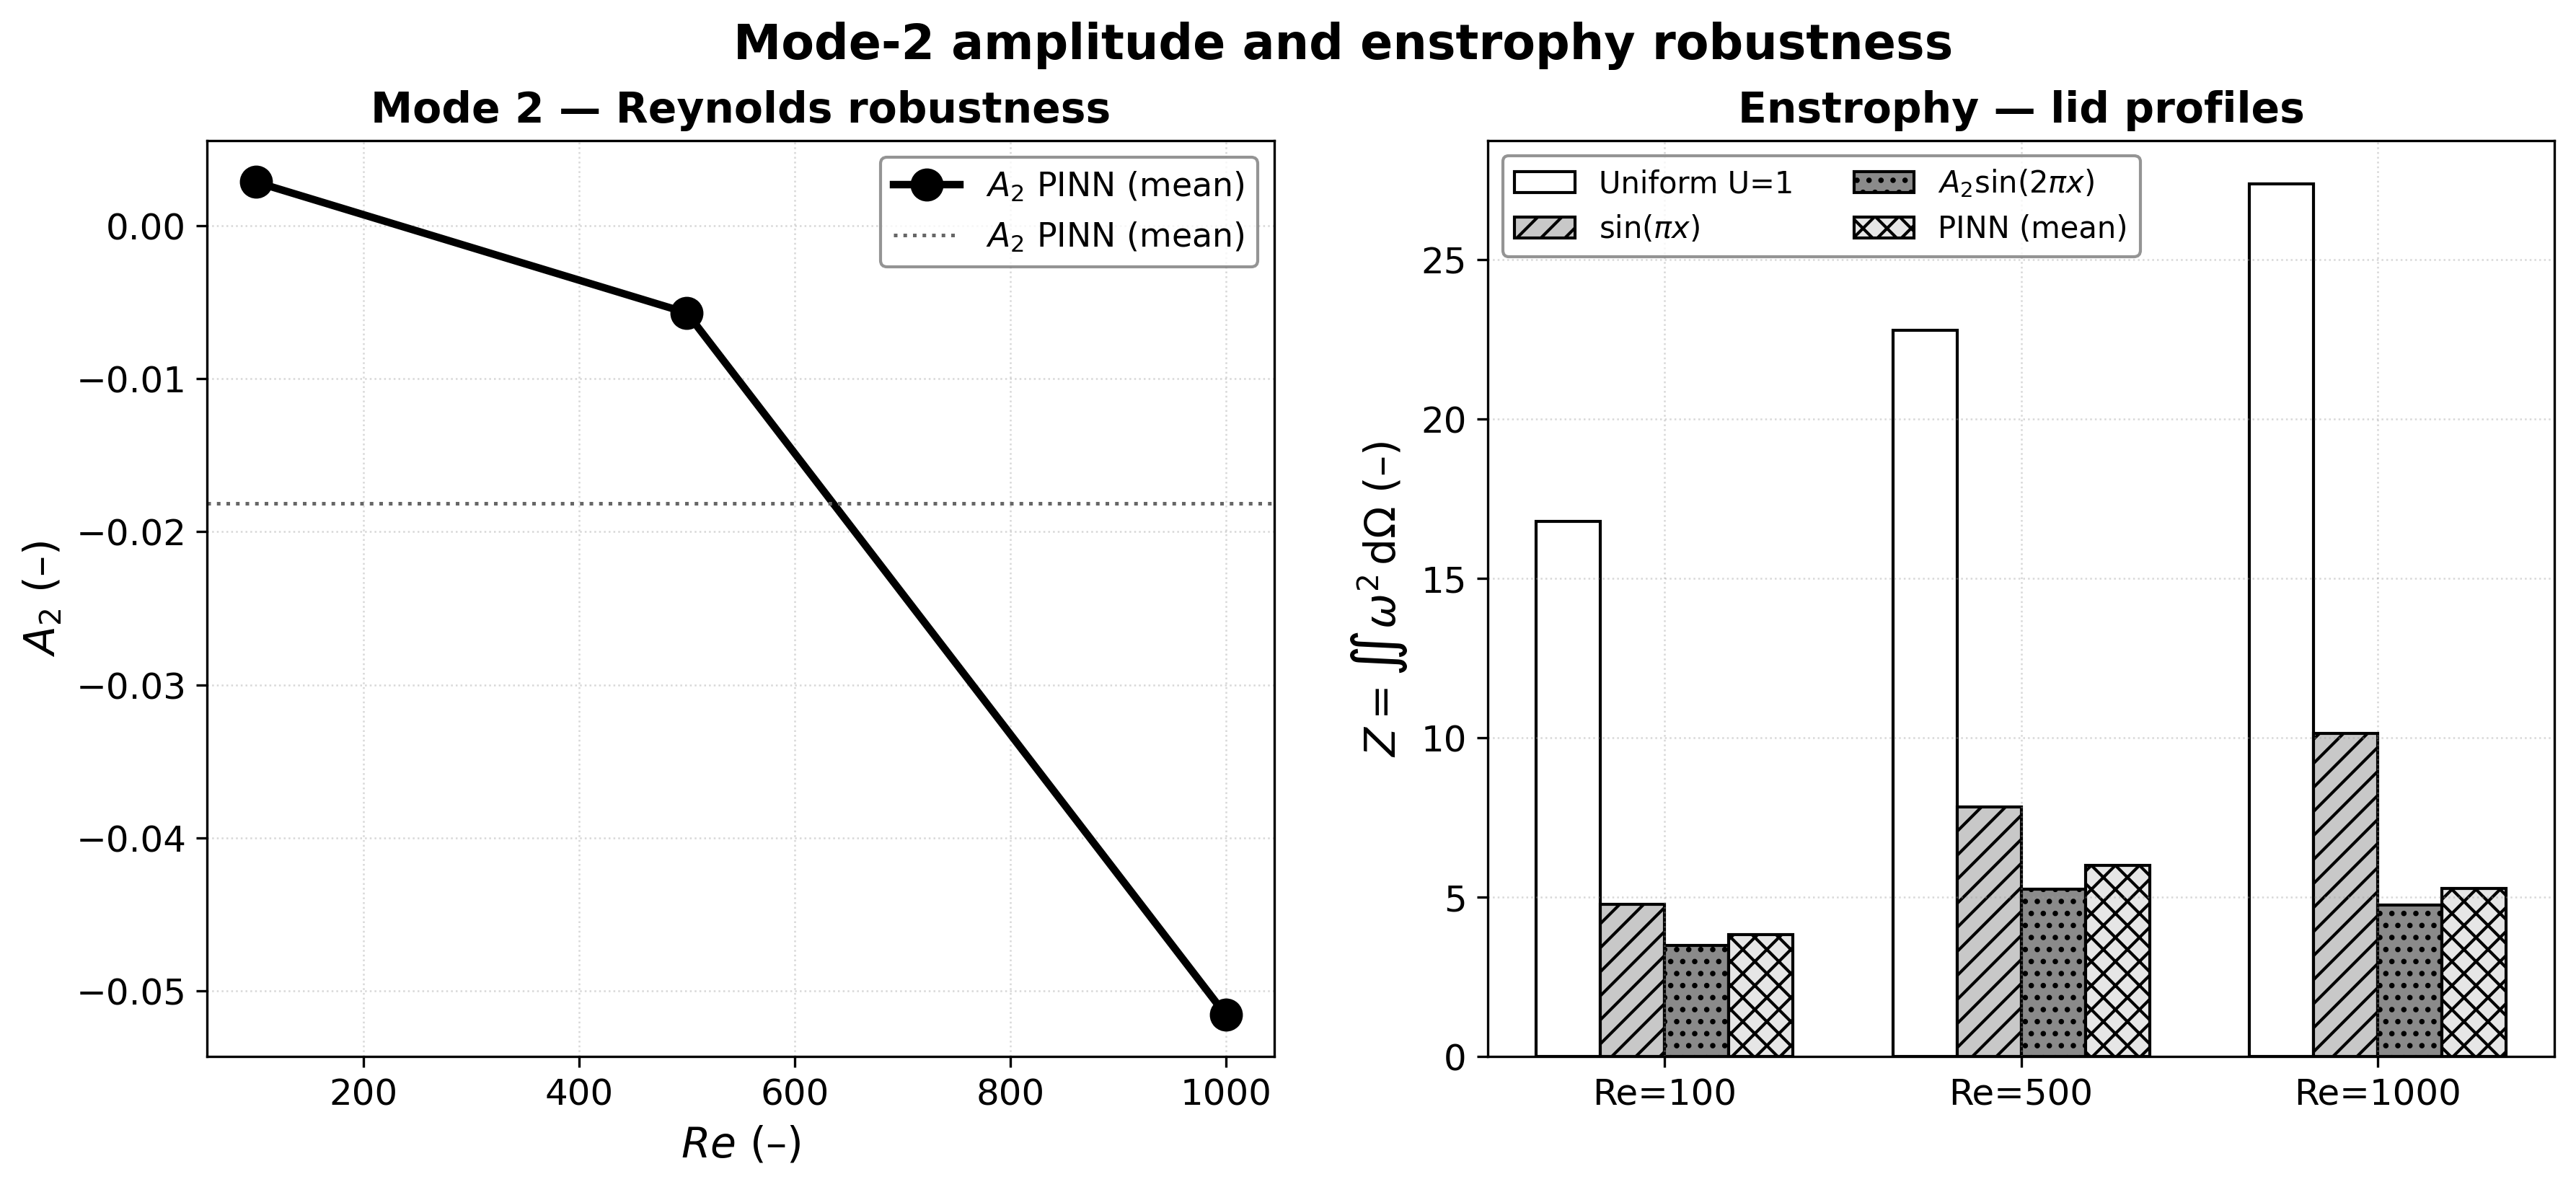
\includegraphics[width=\linewidth]{figures/fig4_reynolds_robustness.png}
\caption{\label{fig:reyn} Reynolds dependence of the flow response to the PINN-identified control, realized in the independent LBM solver. Left: second-mode amplitude $a_2^{\mathrm{flow}}$ of the mean vertical-centerline velocity $u(0.5,y)$ under the PINN (mean) lid profile as a function of $\re$ (open circles) together with its average (dotted line). Right: total enstrophy $Z=\iint\omega^2\,\mathrm{d}\Omega$ for the four lid profiles at each Reynolds number. The controlled branch retains its low-dissipation character across the range, with the degree of modal concentration declining gently from $\re=500$ to $\re=1000$.}
\end{figure}

\subsection{Actuation-energy dependence}\label{sec:energy}

The control-energy sweep at $\re=500$ shows that the second-mode branch is recovered for target energies up to $E^*=0.25$, where the modal concentration is maximal ($f_2=92.5\%$, $f_t=1.2\%$), and that it degrades only for substantially larger targets. For $E^*=0.5$, the second-mode share drops to $85.4\%$ and the temporal content grows to $6.6\%$; for $E^*\ge1.0$ the realized energy saturates around $E_r\approx1$ and the temporal fraction reaches $9.2\%$ ($E^*=1.0$) and $21.8\%$ ($E^*=2.0$). For small targets the realized energy exceeds the target (e.g.\ $E_r=0.0540$ for $E^*=0.01$), because the dissipation term prevents the control from vanishing entirely. The sweep results are collected in Table~\ref{tab:energy} and Fig.~\ref{fig:energysweep}.

\begin{figure}[!t]
\centering
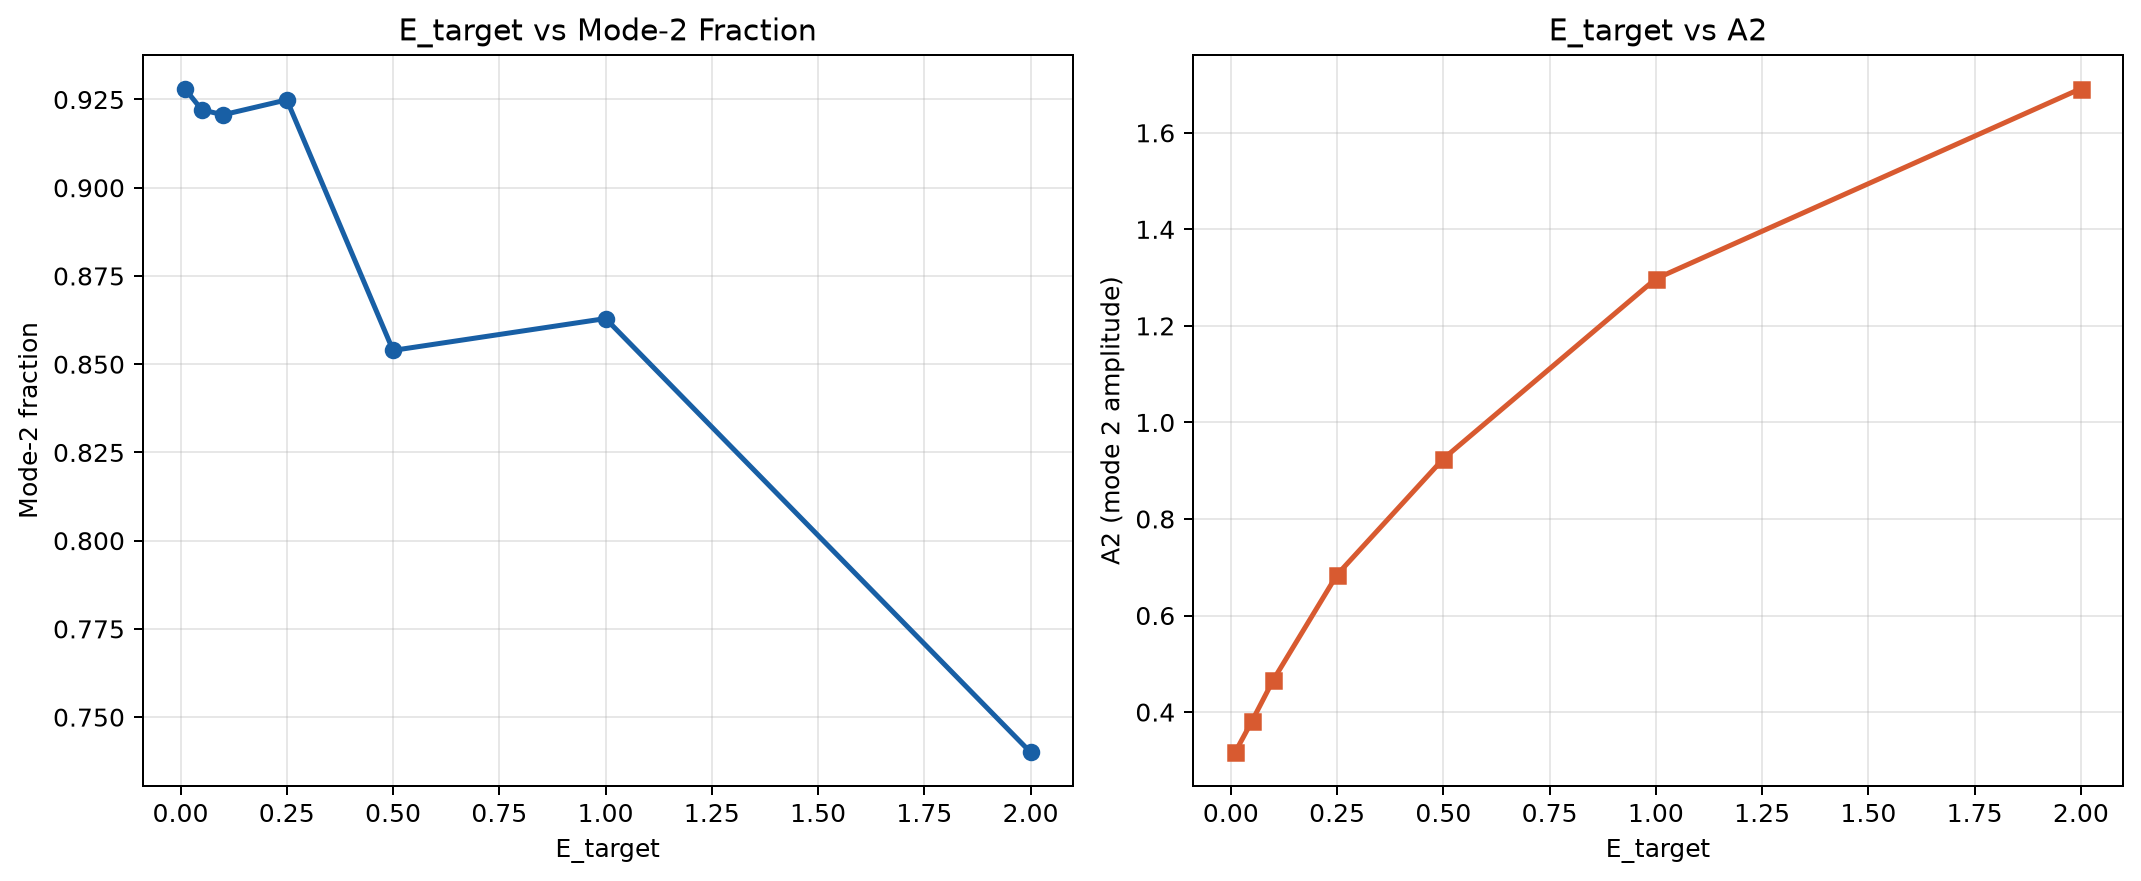
\includegraphics[width=\linewidth]{figures/fig5_energy_sweep.png}
\caption{\label{fig:energysweep} Actuation-energy sweep at $\re=500$, Fourier basis. Left: second-mode energy fraction $f_2$ as a function of the energy target $E^*$. Right: second-mode coefficient $A_2$ as a function of $E^*$. Up to $E^*=0.25$ the modal concentration is maximal; beyond the target $0.5$ the second-mode share degrades and the temporal content grows (see Table~\ref{tab:energy}).}
\end{figure}

\begin{table}[t]
\caption{\label{tab:energy} Actuation-energy sweep at $\re=500$, Fourier basis, seed 42: target $E^*$, realized energy $E_r$, second-mode fraction $f_2$, and temporal fraction $f_t$.}
\centering
\begin{tabular}{cccc}
\toprule
$E^*$ & $E_r$ & $f_2$ (\%) & $f_t$ (\%) \\
\midrule
0.01 & 0.0540 & 92.8 & 0.4 \\
0.05 & 0.0790 & 92.2 & 0.5 \\
0.10 & 0.1183 & 92.1 & 0.7 \\
0.25 & 0.2534 & 92.5 & 1.2 \\
0.50 & 0.5006 & 85.4 & 6.6 \\
1.00 & 0.9756 & 86.3 & 9.2 \\
2.00 & 1.9333 & 74.0 & 21.8 \\
\bottomrule
\end{tabular}
\end{table}

\subsection{Training stochasticity and branch multiplicity}\label{sec:seeds}

The ten seed runs at the nominal settings populate three distinct branches: four runs recover the stationary second-mode branch with $f_2=86.3\%$--$91.3\%$, four runs reach a time-dependent branch with $f_t=97.8\%$--$99.6\%$ and negligible second-mode content, and two runs are intermediate ($f_2\approx52\%$, $f_t\approx44$--45\%). This coexistence shows that the stationary second-mode branch is not the unique minimizer of the multi-objective loss: a subset of random initializations converges to a different, time-dependent branch with a comparable total loss. The seed study is summarized in Table~\ref{tab:seeds}.

\begin{table}[t]
\caption{\label{tab:seeds} Training-stochasticity study at $\re=500$, $E^*=0.25$: seed, realized energy $E_r$, second-mode fraction $f_2$, temporal fraction $f_t$, and final total loss $\mathcal{L}_{\mathrm{tot}}$. Seeds 1, 2, 6, 7 reach the spatial branch ($f_2\ge86\%$); seeds 3, 5, 8, 9 reach the temporal branch ($f_t\ge97\%$); seeds 0 and 4 are intermediate.}
\centering
\begin{tabular}{ccccc}
\toprule
Seed & $E_r$ & $f_2$ (\%) & $f_t$ (\%) & $\mathcal{L}_{\mathrm{tot}}$ \\
\midrule
0 & 0.240 & 53.2 & 43.8 & 1.377 \\
1 & 0.267 & 91.1 & 1.3 & 1.377 \\
2 & 0.257 & 89.2 & 5.0 & 1.374 \\
3 & 0.268 & 2.1 & 97.8 & 1.372 \\
4 & 0.250 & 52.2 & 45.0 & 1.394 \\
5 & 0.245 & 0.4 & 99.5 & 1.373 \\
6 & 0.265 & 86.3 & 1.0 & 1.376 \\
7 & 0.250 & 91.3 & 1.6 & 1.374 \\
8 & 0.250 & 1.3 & 98.4 & 1.372 \\
9 & 0.267 & 0.1 & 99.6 & 1.371 \\
\bottomrule
\end{tabular}
\end{table}

\subsection{Loss ablation and branch selection}\label{sec:ablation}

The loss-ablation study isolates the mechanism that selects the branch by removing or reweighting the loss terms one at a time at the nominal settings (Table~\ref{tab:ablation}). The variance regularizer is the dominant selector: removing it moves the recovered control away from the stationary second-mode branch onto the first spatial harmonic ($f_2\approx0.2\%$, $f_t\approx5.1\%$), whereas strengthening it (weight $\times10$) restores and slightly concentrates the second-mode branch ($f_2\approx92.8\%$). The dissipation and control-energy terms play a secondary, moderating role: removing the dissipation term leaves the second-mode branch essentially unchanged ($f_2\approx92.3\%$, $f_t\approx1.2\%$), and reducing the energy-target weight by half preserves it ($f_2\approx92.5\%$). The ablation therefore attributes the branch selection to the joint action of the dissipation objective (which prefers the smooth, low-dissipation mean state) and the variance regularization (which rejects rapidly varying controls).

\begin{table}[t]
\caption{\label{tab:ablation} Loss-ablation results at $\re=500$, $E^*=0.25$, seed 42: realized energy and modal fractions under removal or reweighting of the loss terms. The baseline rows correspond to the nominal settings.}
\centering
\begin{tabular}{lccc}
\toprule
Config. & $E_r$ & $f_2$ (\%) & $f_t$ (\%) \\
\midrule
Full loss & 0.2534 & 92.2 & 1.2 \\
Variance removed & 0.2582 & 0.2 & 5.1 \\
Variance $\times10$ & 0.2598 & 92.8 & 1.0 \\
Dissipation removed & 0.2533 & 92.3 & 1.2 \\
Energy-target $\times0.5$ & 0.2597 & 92.5 & 1.2 \\
\bottomrule
\end{tabular}
\end{table}

\subsection{Network-capacity and control-space truncation}\label{sec:archmode}

Across the tested network capacities (parameter counts from approximately $9\times10^3$ to $1.4\times10^5$), the realized branch remains the stationary second mode, with $f_2$ between $86\%$ and $94\%$ and $f_t$ below $5\%$; the only deviation is the intermediate seed-0 realization ($f_2\approx53\%$) that belongs to the known intermediate branch of Section~\ref{sec:seeds}. Varying the basis truncation $n_{mx}\times n_{mt}$ over $\{4\times3,\,6\times1,\,6\times3,\,6\times5,\,8\times5,\,8\times9\}$ leaves the dominant mode unchanged, with $f_2$ between $87.3\%$ and $92.3\%$ (Table~\ref{tab:archmode}). The branch is therefore robust to the network capacity and to the basis truncation within the tested ranges.

\begin{table}[t]
\caption{\label{tab:archmode} Control-space truncation and network-capacity robustness at $\re=500$, $E^*=0.25$, seed 42. $E_r$ is the realized energy, $f_2$ and $f_t$ the modal fractions. All configurations are retrained from scratch.}
\centering
\begin{tabular}{lccccc}
\toprule
$n_{mx}\times n_{mt}$ & $n_{\mathrm{modes}}$ & $E_r$ & $f_2$ (\%) & $f_t$ (\%) & Dominant \\
\midrule
$4\times3$ & 12 & 0.2586 & 91.2 & 0.9 & $(2,0)$ \\
$6\times1$ & 6 & 0.2390 & 89.2 & 0.0 & $(2,0)$ \\
$6\times3$ & 18 & 0.2778 & 89.3 & 1.3 & $(2,0)$ \\
$6\times5$ & 30 & 0.2533 & 92.3 & 1.2 & $(2,0)$ \\
$8\times5$ & 40 & 0.2475 & 87.8 & 1.5 & $(2,0)$ \\
$8\times9$ & 72 & 0.2775 & 87.3 & 2.9 & $(2,0)$ \\
\bottomrule
\end{tabular}
\end{table}

\subsection{Aspect-ratio dependence}\label{sec:ar}

The aspect-ratio sweep repeats the branch analysis for a $2{:}1$ rectangular cavity at the nominal settings. The stationary second-mode branch persists: the realized energy changes by less than $1\%$ ($E_r=0.2514$), the second-mode fraction varies from $92.2\%$ (square) to $91.2\%$ (rectangular), and the coefficient $A_2$ from $0.6835$ to $0.6770$, with a modest growth of the temporal content from $1.2\%$ to $1.6\%$. The results are shown in Table~\ref{tab:ar} and Fig.~\ref{fig:ar}.

\begin{figure}[!t]
\centering
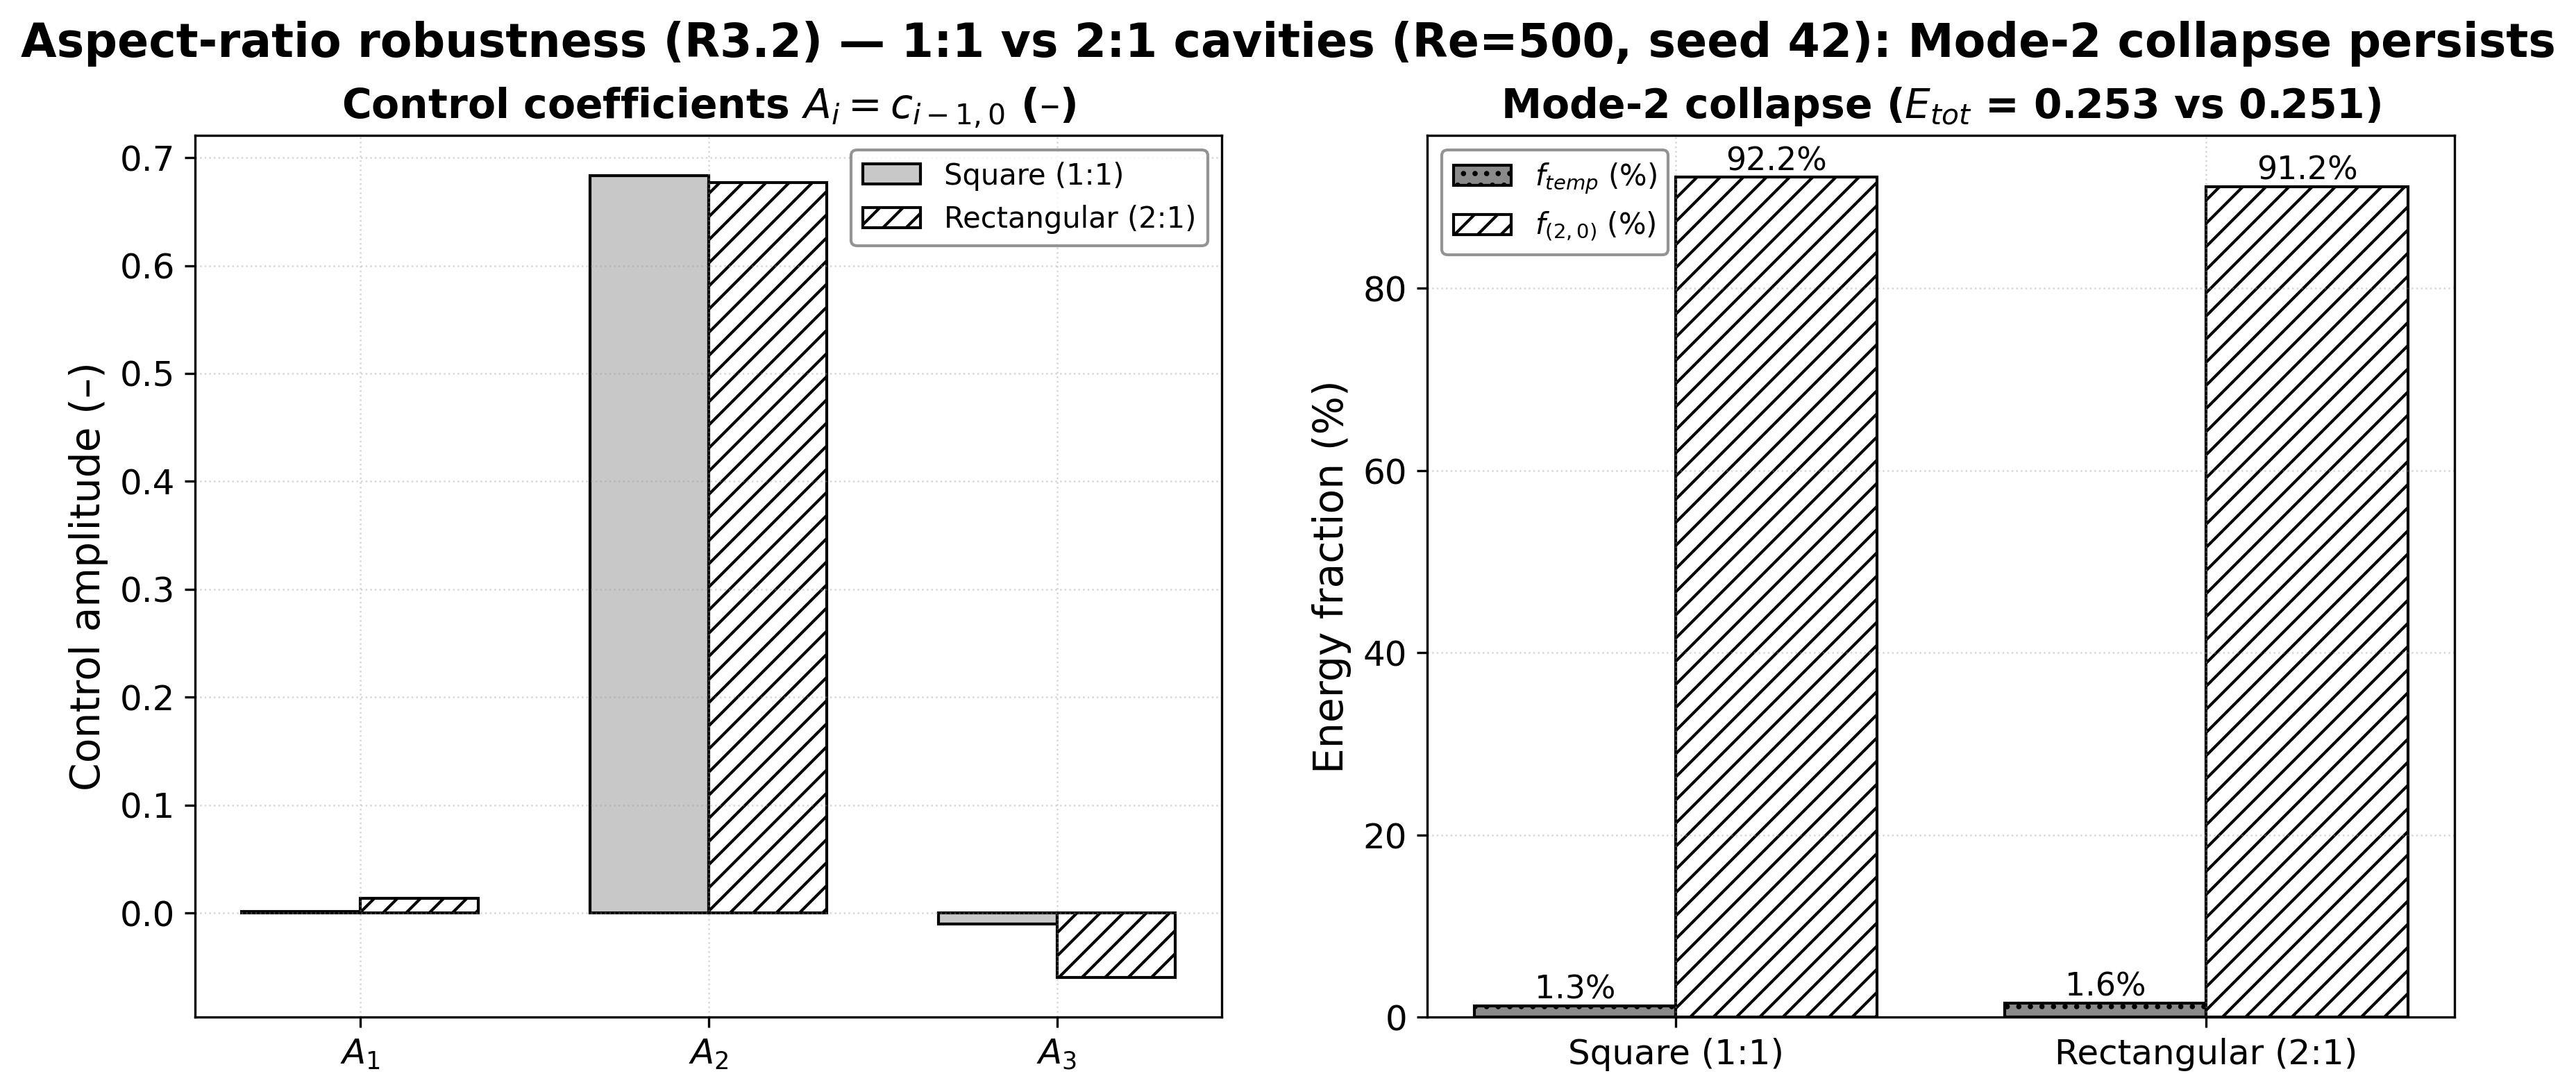
\includegraphics[width=\linewidth]{figures/fig6_aspect_ratio.png}
\caption{\label{fig:ar} Aspect-ratio robustness at $\re=500$, seed 42, $E^*=0.25$. Left: control coefficients $A_1$, $A_2$, $A_3$ for the square (1:1) and rectangular (2:1) cavities. Right: second-mode fraction $f_{(2,0)}$ and temporal fraction $f_t$ for the two geometries. The second-mode branch persists in the $2{:}1$ cavity, with $f_2$ varying from $92.2\%$ to $91.2\%$ and the realized energy changing by less than $1\%$.}
\end{figure}

\begin{table}[t]
\caption{\label{tab:ar} Aspect-ratio robustness at $\re=500$, $E^*=0.25$, seed 42: coefficient $A_2$, realized energy $E_r$, and modal fractions for the square ($1{:}1$) and rectangular ($2{:}1$) cavities.}
\centering
\begin{tabular}{lcccc}
\toprule
Geometry & $A_2$ & $E_r$ & $f_2$ (\%) & $f_t$ (\%) \\
\midrule
Square ($1{:}1$) & 0.6835 & 0.2534 & 92.2 & 1.2 \\
Rectangular ($2{:}1$) & 0.6770 & 0.2514 & 91.2 & 1.6 \\
\bottomrule
\end{tabular}
\end{table}

The structure of the identified control is quantitatively similar in both cavities. Figure~\ref{fig:lidprofiles} compares the complete PINN control with its dominant-mode truncation and with the reference pure sinusoid $A_2\sin(2\pi s)$ for the two geometries: the agreement between the three profiles shows that the identified control is close to its dominant-mode truncation, even when the cavity is elongated.

\begin{figure}[!t]
\centering
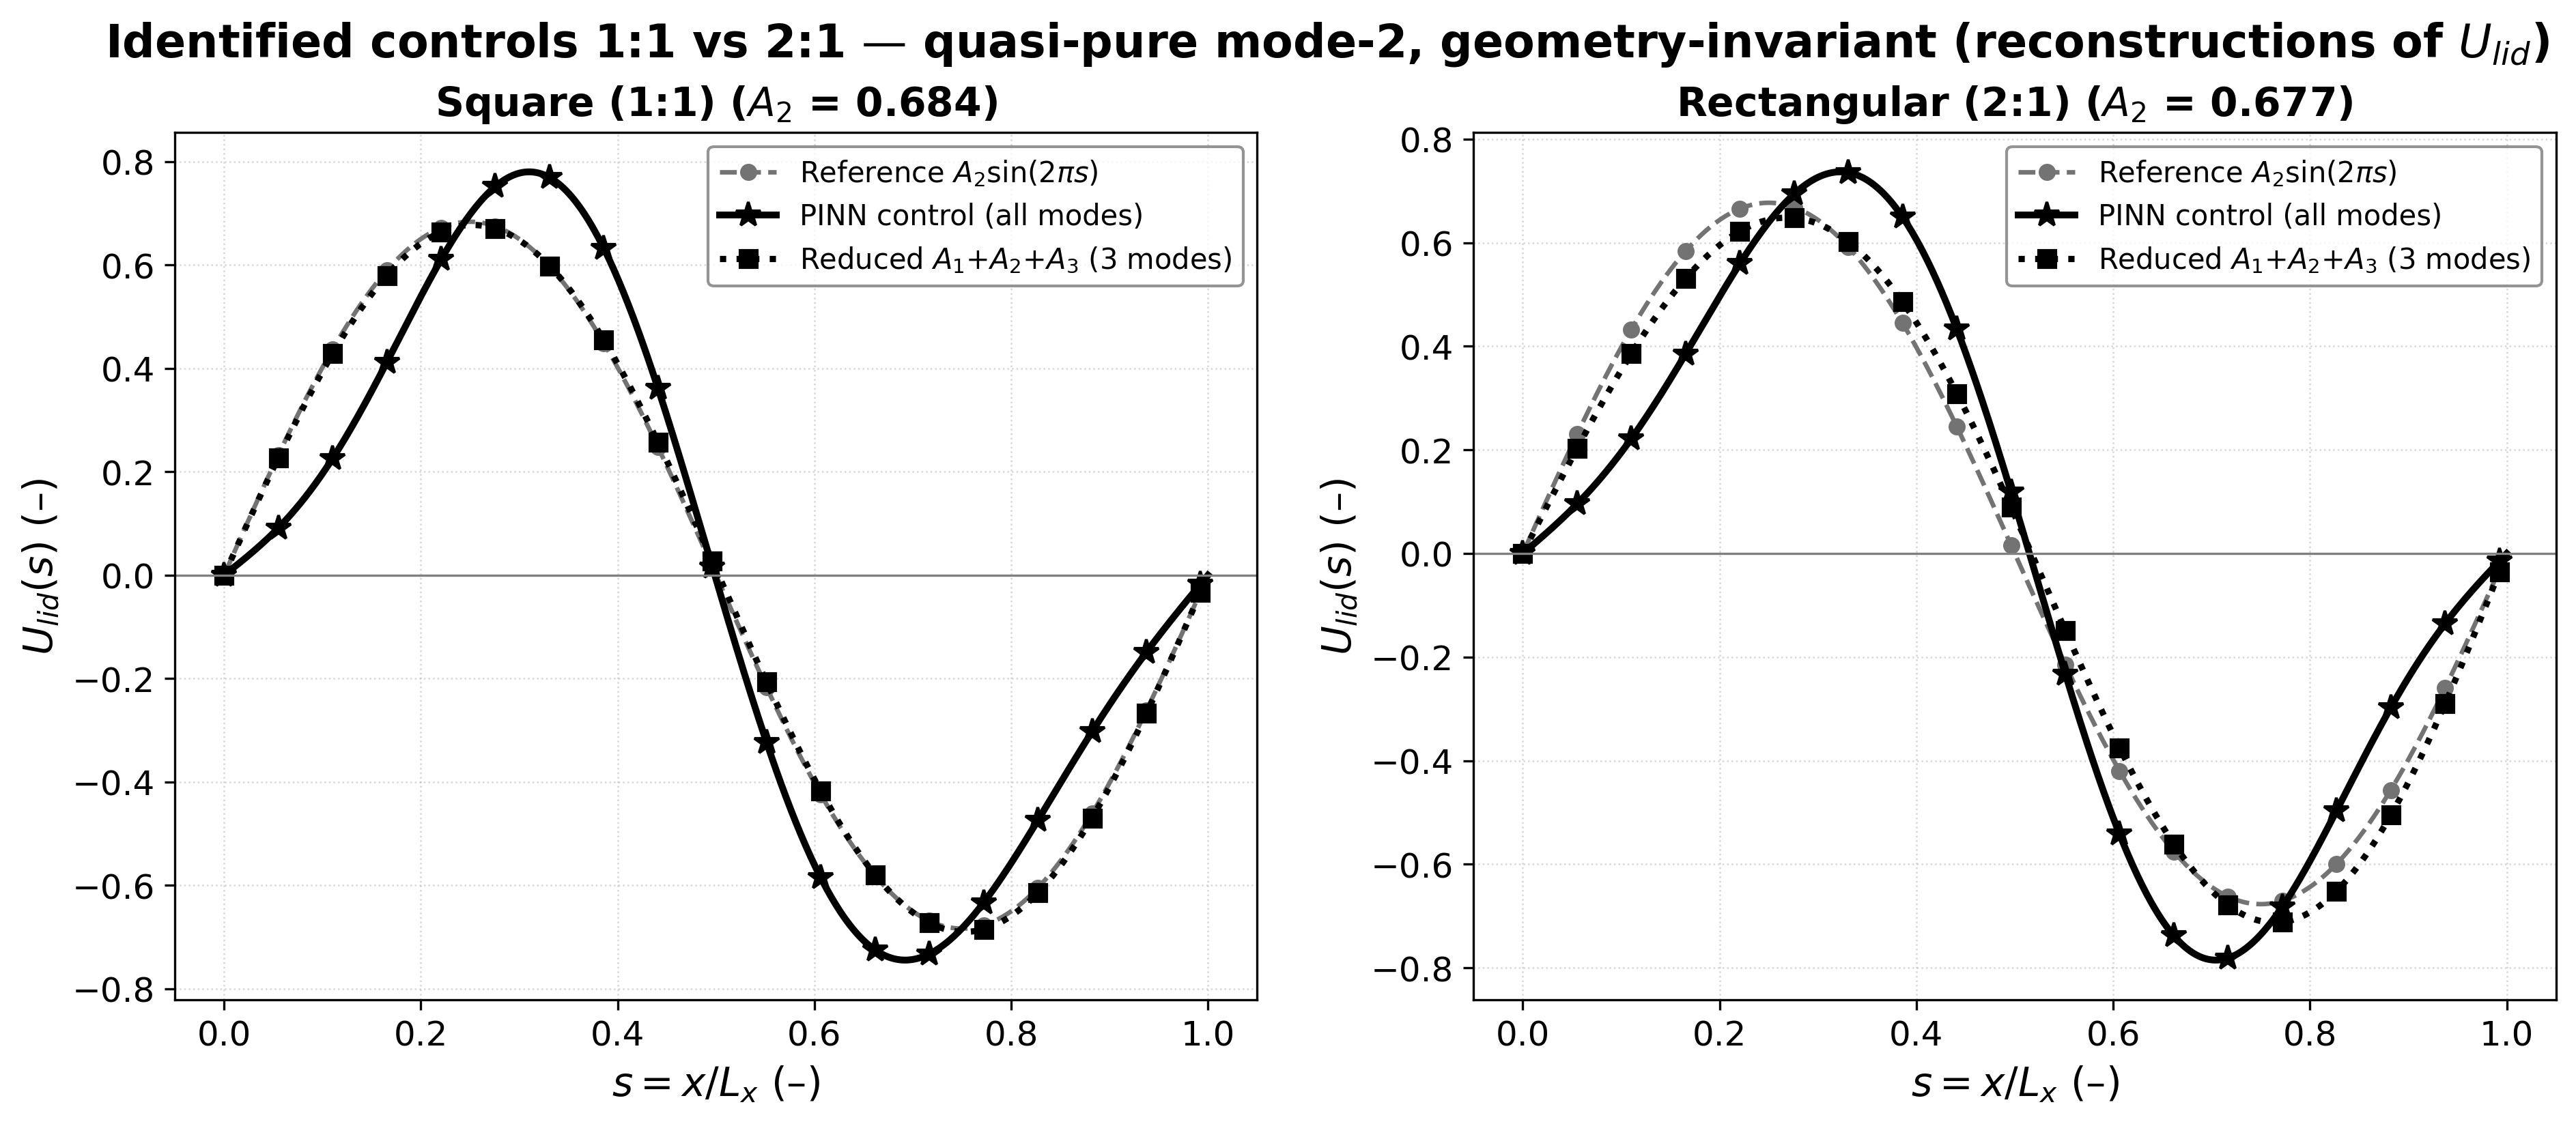
\includegraphics[width=\linewidth]{figures/fig7_lid_profiles.png}
\caption{\label{fig:lidprofiles} Identified lid controls $U_{\mathrm{lid}}(s)$ with $s=x/L_x$ for the square (left) and $2{:}1$ (right) cavities at $\re=500$: reference $A_2\sin(2\pi s)$ (dashed, open symbols), complete PINN control (solid), and reduced three-mode reconstruction (dotted). The coincidence of the three curves shows that the identified control is quantitatively close to its dominant-mode truncation.}
\end{figure}

\subsection{Control-parametrization dependence}\label{sec:param}

The basis comparison drives the main conclusion of the parametrization study. The PINN-identified Fourier control realizes the target with $f_2\simeq92\%$ and $f_t\simeq1\%$ at $\re=500$; the modified-Chebyshev control, trained with the same capacity and the same settings, realizes a temporally dominated control (Table~\ref{tab:param}). Because the realized energies of the two parametrizations differ ($E_r\simeq0.253$--$0.269$ for the Fourier branch versus $0.285$--$0.291$ for the Chebyshev branch), the comparison is not an exactly matched-energy experiment: we therefore compare the structure and the admissibility of the two branches, not their dissipation at equal energy. This difference is not an artifact of the training: the two controls have comparable total loss, and both are evaluated in the independent solver. The Fourier and Chebyshev branches therefore differ in their admissibility: the Fourier branch is quasi-stationary ($R_K<1\%$), whereas the Chebyshev branch is not (Section~\ref{sec:cheb_lbm}). The comparison tones down the physical interpretation of the branch: the recovered second-mode control is a property of the identification problem under the Fourier parametrization, not a universal feature of the physics.

\begin{table}[t]
\caption{\label{tab:param} Control-parametrization comparison at $\re=100,500,1000$: realized energy $E_r$, second-mode coefficient $A_2$, second-mode fraction $f_2$, and temporal fraction $f_t$, for the Fourier and modified-Chebyshev parametrizations. $A_2$ refers to the amplitude of the stationary second mode in the Fourier projection.}
\centering
\begin{tabular}{lcccc}
\toprule
Parametrization & $\re$ & $E_r$ & $A_2$ & $f_2$ (\%) \\
\midrule
Fourier & 100 & 0.2581 & 0.6876 & 91.6 \\
Fourier & 500 & 0.2534 & 0.6835 & 92.2 \\
Fourier & 1000 & 0.2687 & 0.5863 & 64.0 \\
\midrule
Chebyshev & 100 & 0.2890 & $-0.039$ & 0.3 \\
Chebyshev & 500 & 0.2850 & $-0.187$ & 6.2 \\
Chebyshev & 1000 & 0.2908 & $-0.053$ & 0.5 \\
\bottomrule
\end{tabular}
\end{table}

\subsection{Independent LBM solver verification}\label{sec:ghia}

The LBM solver is first validated on the classical uniform-lid cavity. The mean horizontal velocity $u(0.5,y)$ along the vertical centerline matches the reference data of Ghia \emph{et al.}~\cite{ghia1982high} at $\re=100$ and $\re=1000$ ($L_2$ error below $1.5\%$ on the centerline). The comparison is shown in Fig.~\ref{fig:ghia}.

\begin{figure}[!t]
\centering
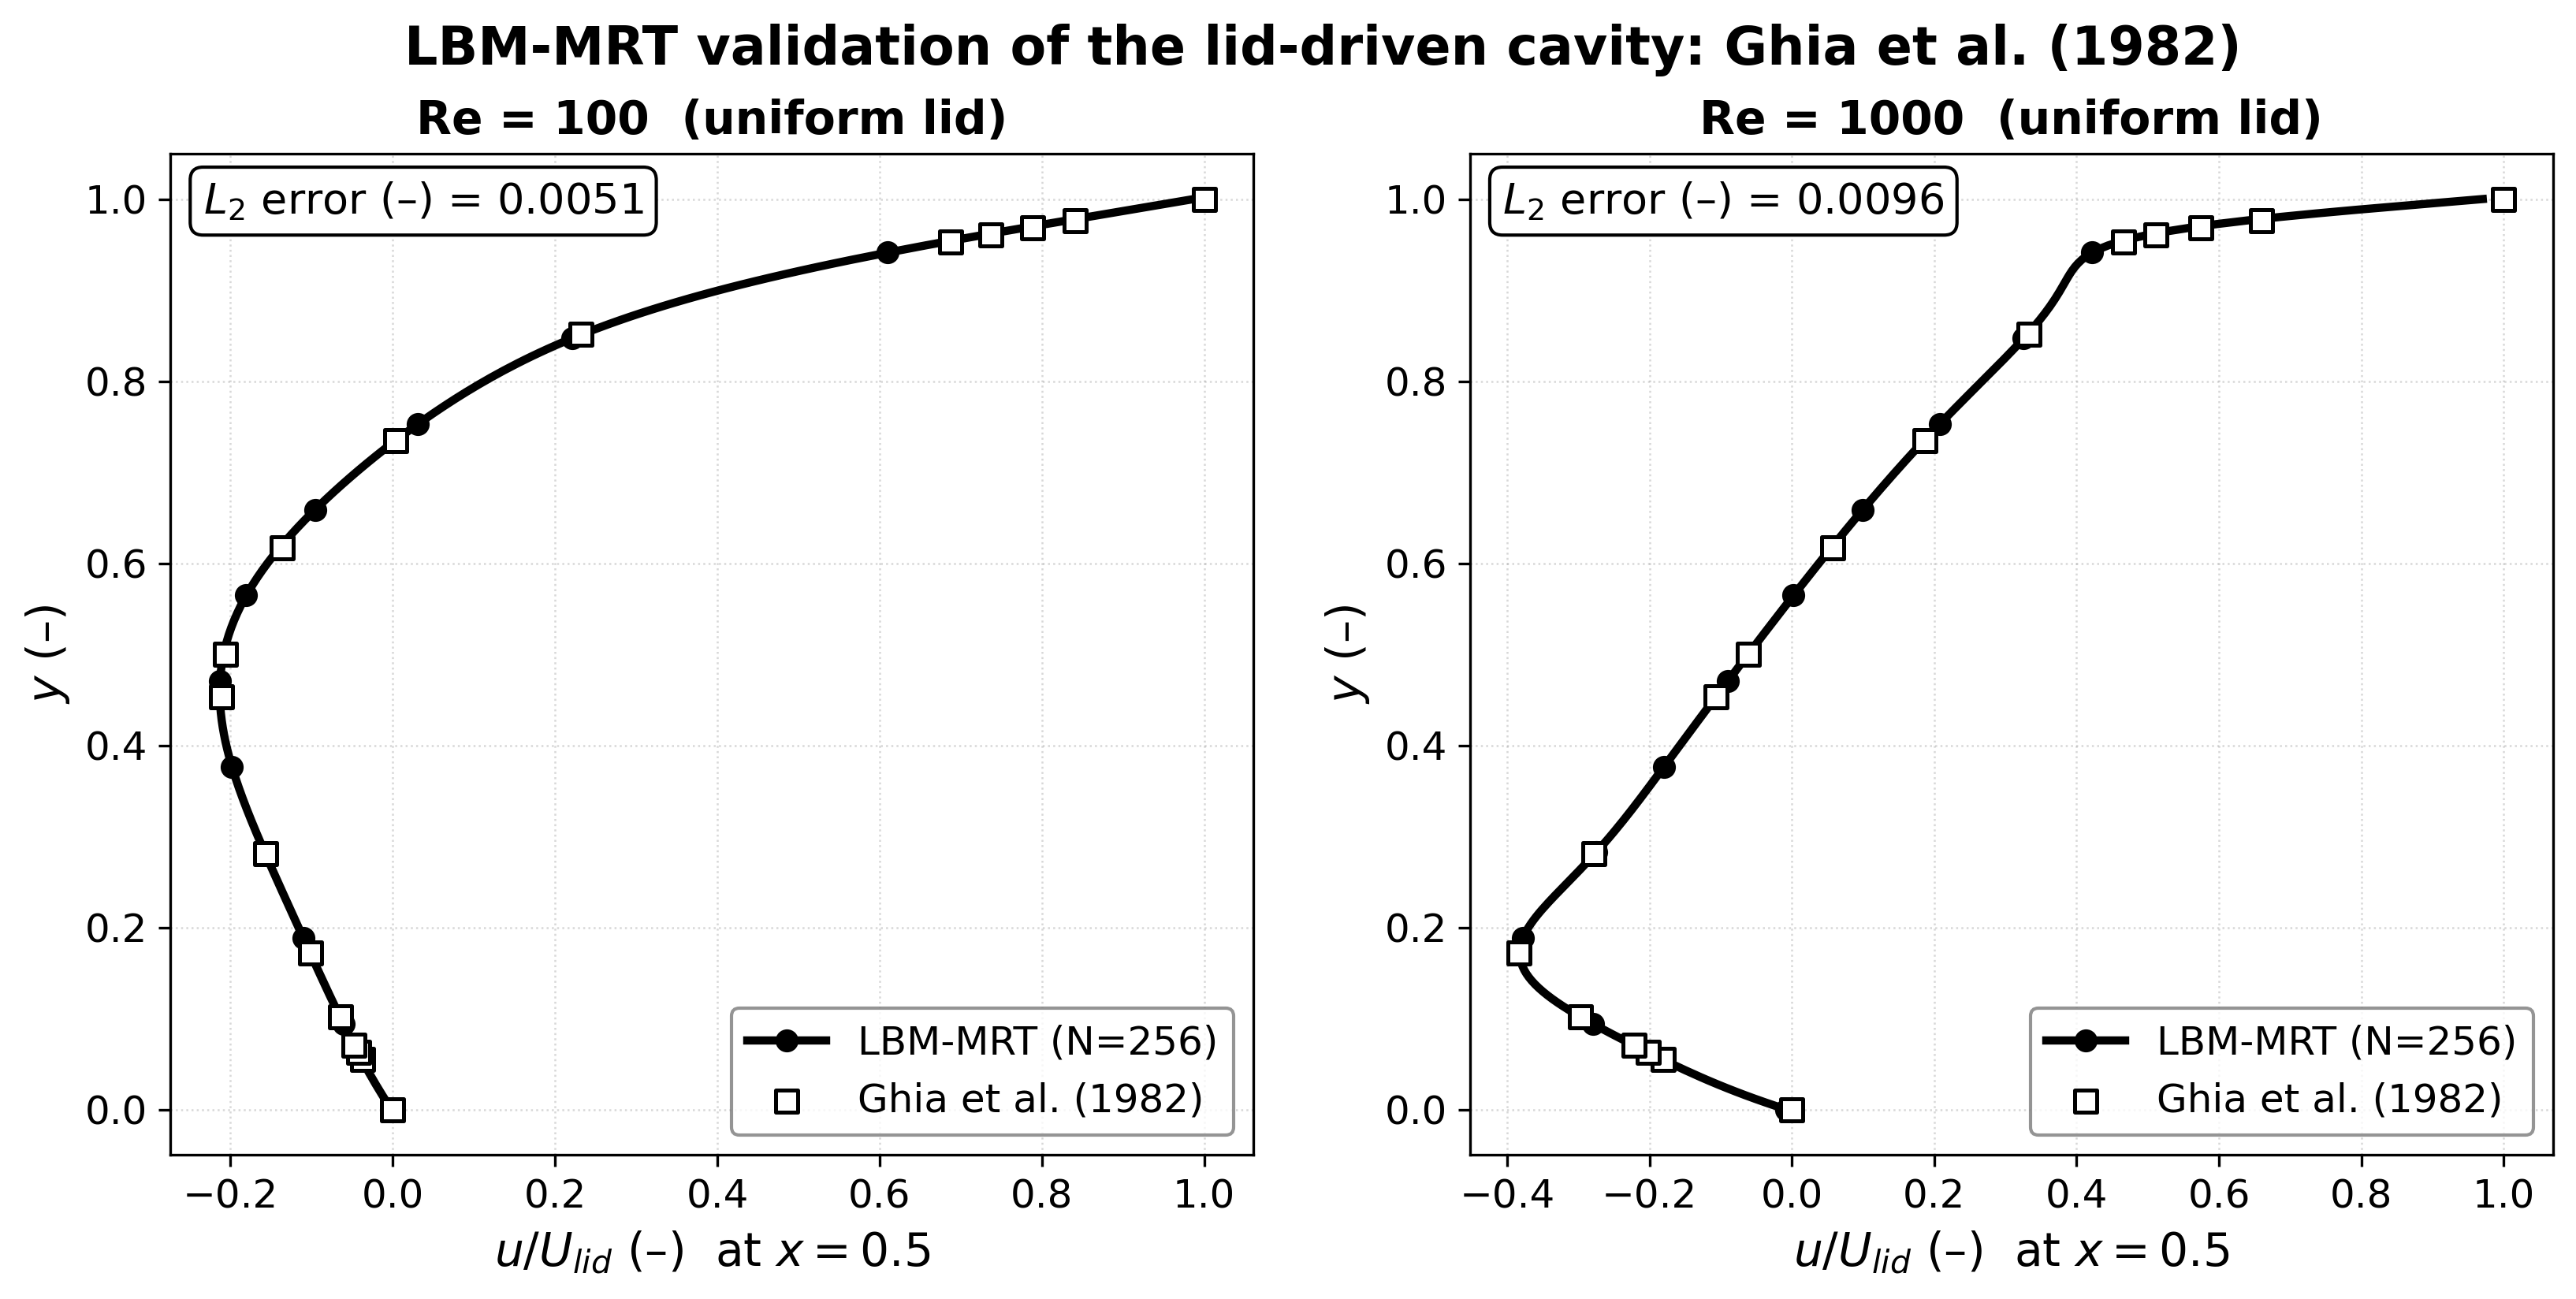
\includegraphics[width=\linewidth]{figures/fig8_lbm_ghia.png}
\caption{\label{fig:ghia} Validation of the independent LBM-MRT solver against the reference data of Ghia \emph{et al.}~\cite{ghia1982high} for the standard uniform-lid cavity at $\re=100$ and $\re=1000$. The mean horizontal velocity $u(0.5,y)$ is shown with the reference points; the reported $L_2$ error is computed on the vertical centerline.}
\end{figure}

\subsection{Grid convergence and discretization uncertainty}\label{sec:gci}

The grid-dependence of the dissipation metric is characterized at $\re=500$ under the $A_2\sin(2\pi x)$ control on grids of $N=128$, $256$, and $512$ points. The integrated dissipation $\varepsilon$ converges monotonically ($\varepsilon=0.00935,0.01041,0.01091$), the Richardson extrapolation gives $p=1.08$ and the extrapolated value $\varepsilon^*=0.0114$, and the grid-convergence index is approximately $11\%$ at the production resolution $N=256$ and $5\%$ at $N=512$. The reduction achieved by the second-mode control with respect to the uniform lid ($73$--$80\%$ across the Reynolds range) therefore far exceeds the discretization uncertainty, whereas the smaller difference between the complete PINN control and its dominant-mode truncation is of the same order as that uncertainty and is not further interpreted as resolved.

\subsection{Independent verification of the Fourier branch}\label{sec:dissipation}

The complete PINN control and its dominant-mode truncation are applied in the LBM solver at the realized amplitude. Two robust quantitative findings emerge. First, the dissipation reduction of the realized flows relative to the uniform-lid reference is large and consistent: the PINN-identified control yields a dissipation reduction of $77\%$, $73\%$, and $80\%$ at $\re=100$, $500$, and $1000$, its dominant-mode truncation $A_2\sin(2\pi x)$ attains the lowest computed dissipation among the tested profiles at every Reynolds number, and the pure first harmonic $\sin(\pi x)$ is intermediate (Table~\ref{tab:dissipation}, Fig.~\ref{fig:dissipation}). The separation between the complete control and its truncation is within the discretization uncertainty quantified in Section~\ref{sec:gci} and is not interpreted as a resolved ordering. Second, the second-mode response is insensitive to the truncation of the control: $a_2^{\mathrm{flow}}$ extracted from the realized mean flows tracks $a_2^{\mathrm{ctrl}}$ of the PINN control in trend, confirming that the second-mode hypothesis is self-consistent in the independent solver.

\begin{table}[t]
\caption{\label{tab:dissipation} Integrated dissipation $\varepsilon$ of the realized flows from the independent LBM solver ($256\times256$ grid) for the uniform, $\sin(\pi x)$, $A_2\sin(2\pi x)$, and PINN (mean) lid profiles at $\re=100$, $500$, and $1000$.}
\centering
\begin{tabular}{ccccc}
\toprule
$\re$ & Uniform & $\sin(\pi x)$ & $A_2\sin(2\pi x)$ & PINN (mean) \\
\midrule
100  & 0.16195 & 0.04758 & 0.03445 & 0.03776 \\
500  & 0.04425 & 0.01561 & 0.01041 & 0.01189 \\
1000 & 0.02654 & 0.01011 & 0.00473 & 0.00524 \\
\bottomrule
\end{tabular}
\end{table}

\begin{figure}[!t]
\centering
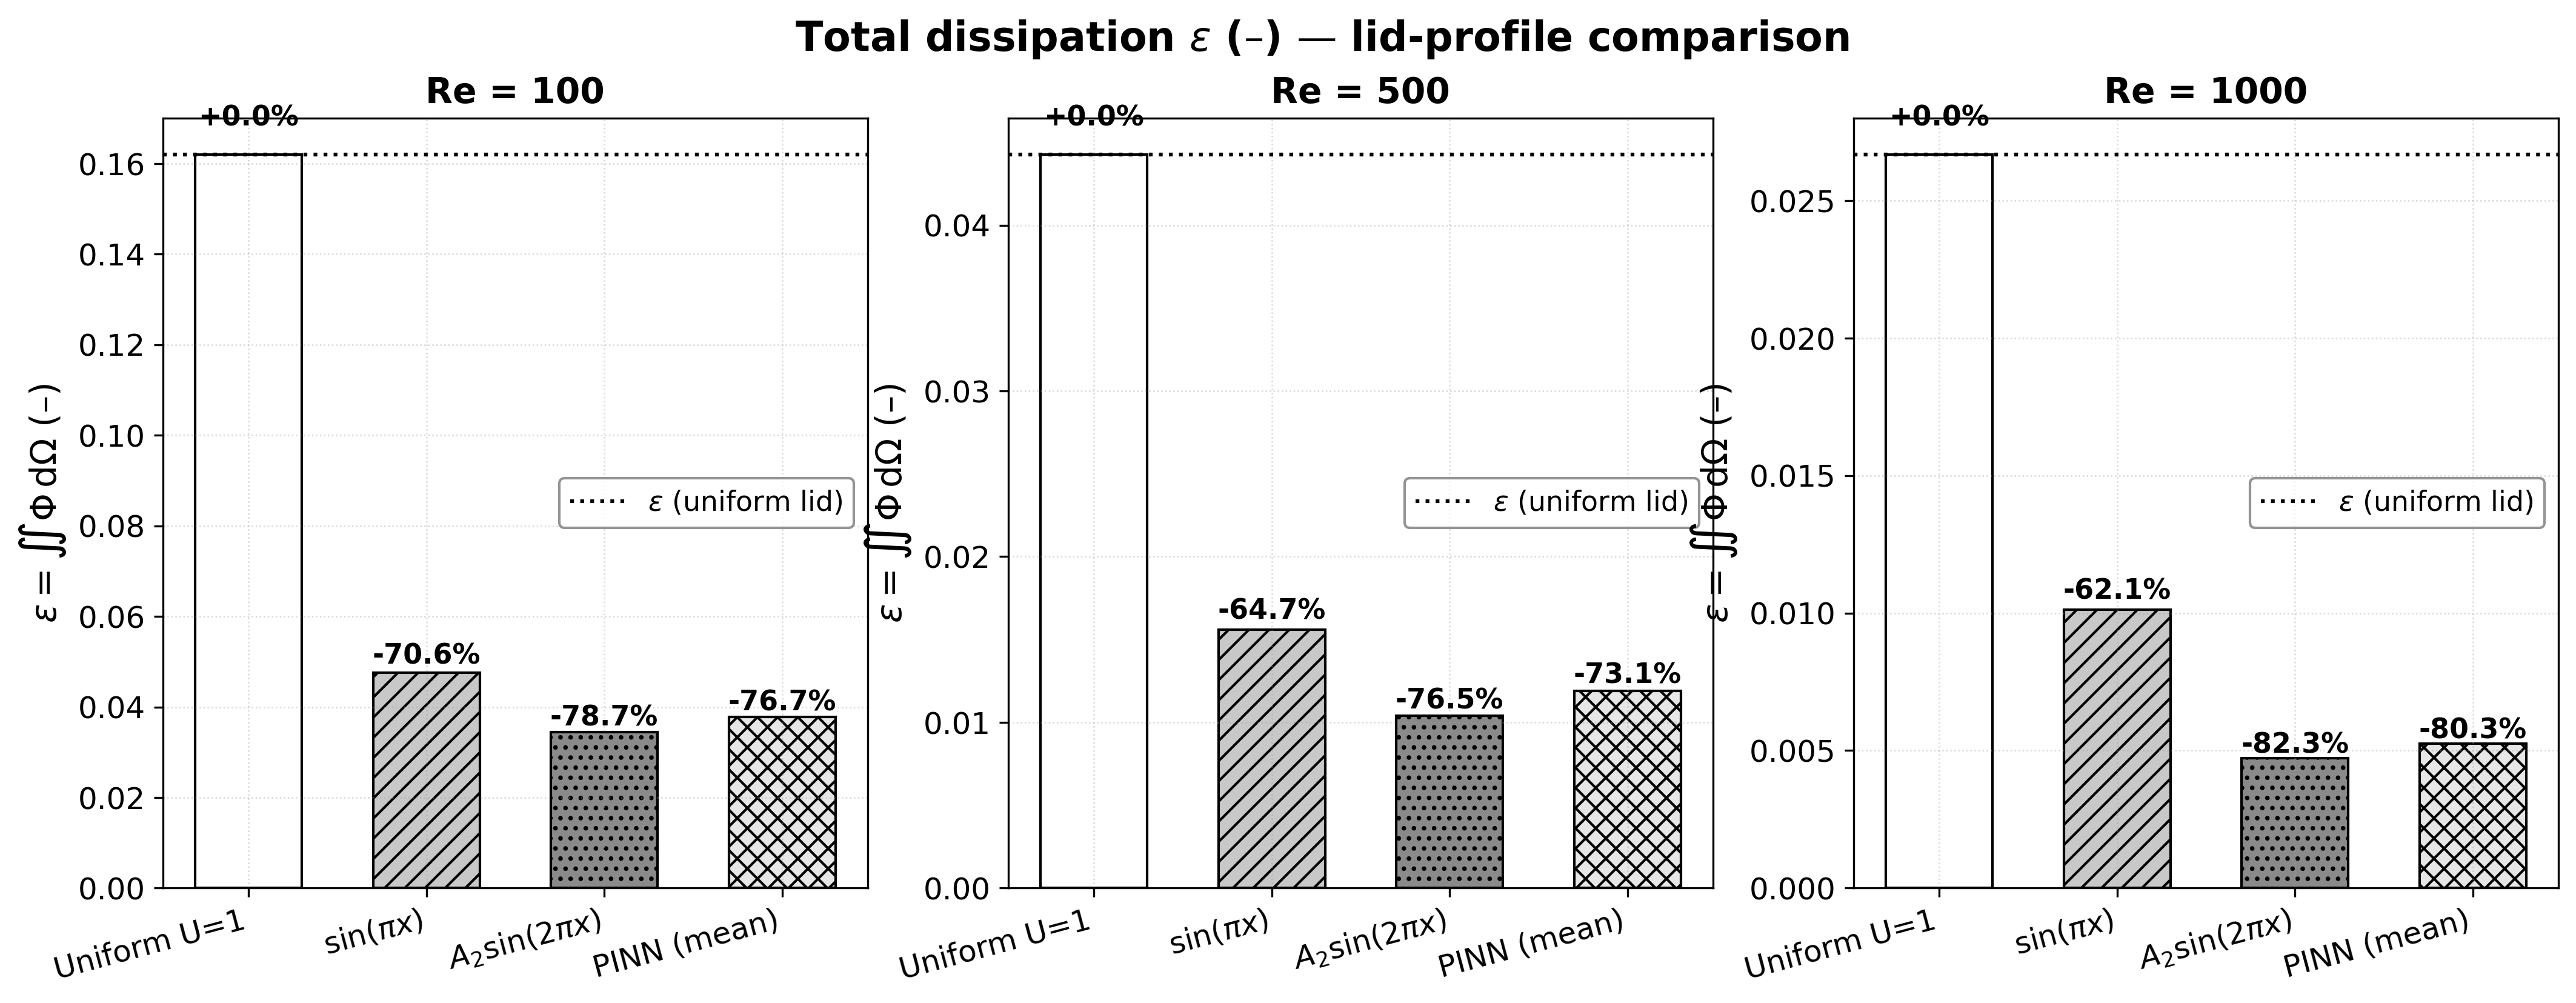
\includegraphics[width=\linewidth]{figures/fig10_dissipation.png}
\caption{\label{fig:dissipation} Integrated dissipation $\varepsilon$ of the realized flows under the four lid profiles at $\re=100$, $500$, and $1000$, from the independent LBM solver. Percentages indicate the relative change with respect to the uniform lid. The complete PINN control and its dominant-mode truncation $A_2\sin(2\pi x)$ achieve the lowest computed dissipation among the tested controls at every Reynolds number; their mutual separation is within the production-grid discretization uncertainty (Section~\ref{sec:gci}).}
\end{figure}

\subsection{Time-dependent LBM assessment of the Fourier branch}\label{sec:fourier_admis}

The temporal assessment of the Fourier branch covers the converged (steady) and the time-resolved stages of the LBM integration. At the realized operating point the second-mode content of the mean flow is stable and the parameter-free projection of the Fourier branch onto the admissibility metric gives $R_K$ at the $0.15\%$, $0.04\%$, and $0.65\%$ level at $\re=100$, $500$, and $1000$ (Table~\ref{tab:admis}), i.e.\ below the $1\%$ threshold of Section~\ref{sec:stationarity}. The small residual fluctuation is concentrated in the harmonics of the window, and the mean-flow diagnostics are therefore representative of the quasi-stationary regime.

\begin{table}[t]
\caption{\label{tab:admis} Admissibility of the Fourier and Chebyshev branches in the independent time-dependent LBM assessment: fluctuating-to-mean-flow kinetic-energy ratio $R_K$ over the window, at $\re=100$, $500$, $1000$. The threshold is $R_K^*=1\%$.}
\centering
\begin{tabular}{lcc}
\toprule
Branch & $\re$ & $R_K$ (\%) \\
\midrule
Fourier & 100 & 0.15 \\
Fourier & 500 & 0.04 \\
Fourier & 1000 & 0.65 \\
\midrule
Chebyshev & 100 & 847 \\
Chebyshev & 500 & 44 \\
Chebyshev & 1000 & 125 \\
\bottomrule
\end{tabular}
\end{table}

\subsection{LBM assessment of the modified-Chebyshev branch}\label{sec:cheb_lbm}

The modified-Chebyshev branch is assessed with the same protocol. Its realized controls are temporally dominated (Table~\ref{tab:param}), and their time-resolved solutions are strongly fluctuating: the fluctuating-to-mean-flow kinetic-energy ratio is $R_K=847\%$, $44\%$, and $125\%$ at $\re=100$, $500$, and $1000$ (Table~\ref{tab:admis}), i.e.\ well above the $1\%$ threshold. The Chebyshev branch therefore fails the operational quasi-stationarity criterion of Section~\ref{sec:stationarity} and is classified as non-admissible. The exceptionally large value at $\re=100$ reflects the very small mean-flow kinetic energy realized by that control at the low Reynolds number: $K_{\mathrm{mean}}$ is of order $10^{-4}$ while $K_{\mathrm{fluct}}$ is of order $10^{-1}$, so the ratio is large although the absolute fluctuation level remains moderate. This interpretation is illustrated by the dissipation and modal-content metrics in the consolidated comparison of Fig.~\ref{fig:consolidated}.

\subsection{Consolidated interpretation}\label{sec:consolidated}

Figure~\ref{fig:consolidated} consolidates the identification and verification campaigns. Panel (a) shows the integrated dissipation of the realized flows under the $A_2\sin(2\pi x)$ control, the complete PINN control, and the uniform reference, versus the Reynolds number: the controlled branch is robustly low-dissipation. Panel (b) compares the control coefficient $a_2^{\mathrm{ctrl}}$ of the PINN representation with the flow response $a_2^{\mathrm{flow}}$ extracted from the LBM mean fields, including the square and $2{:}1$ aspect-ratio values: the two quantities track each other, confirming that the second-mode hypothesis is quantitatively consistent between the identification and the verification stages. Panel (c) shows the admissibility ratio $R_K$ for the Fourier and Chebyshev branches, with the $1\%$ threshold, and panel (d) the dominant modes of the mean fields and of the fluctuations. The consolidated picture is that the Fourier branch passes the admissibility test while the Chebyshev branch fails it, and that the identification is structurally sensitive to the parametrization of the control.

\begin{figure*}[!t]
\centering
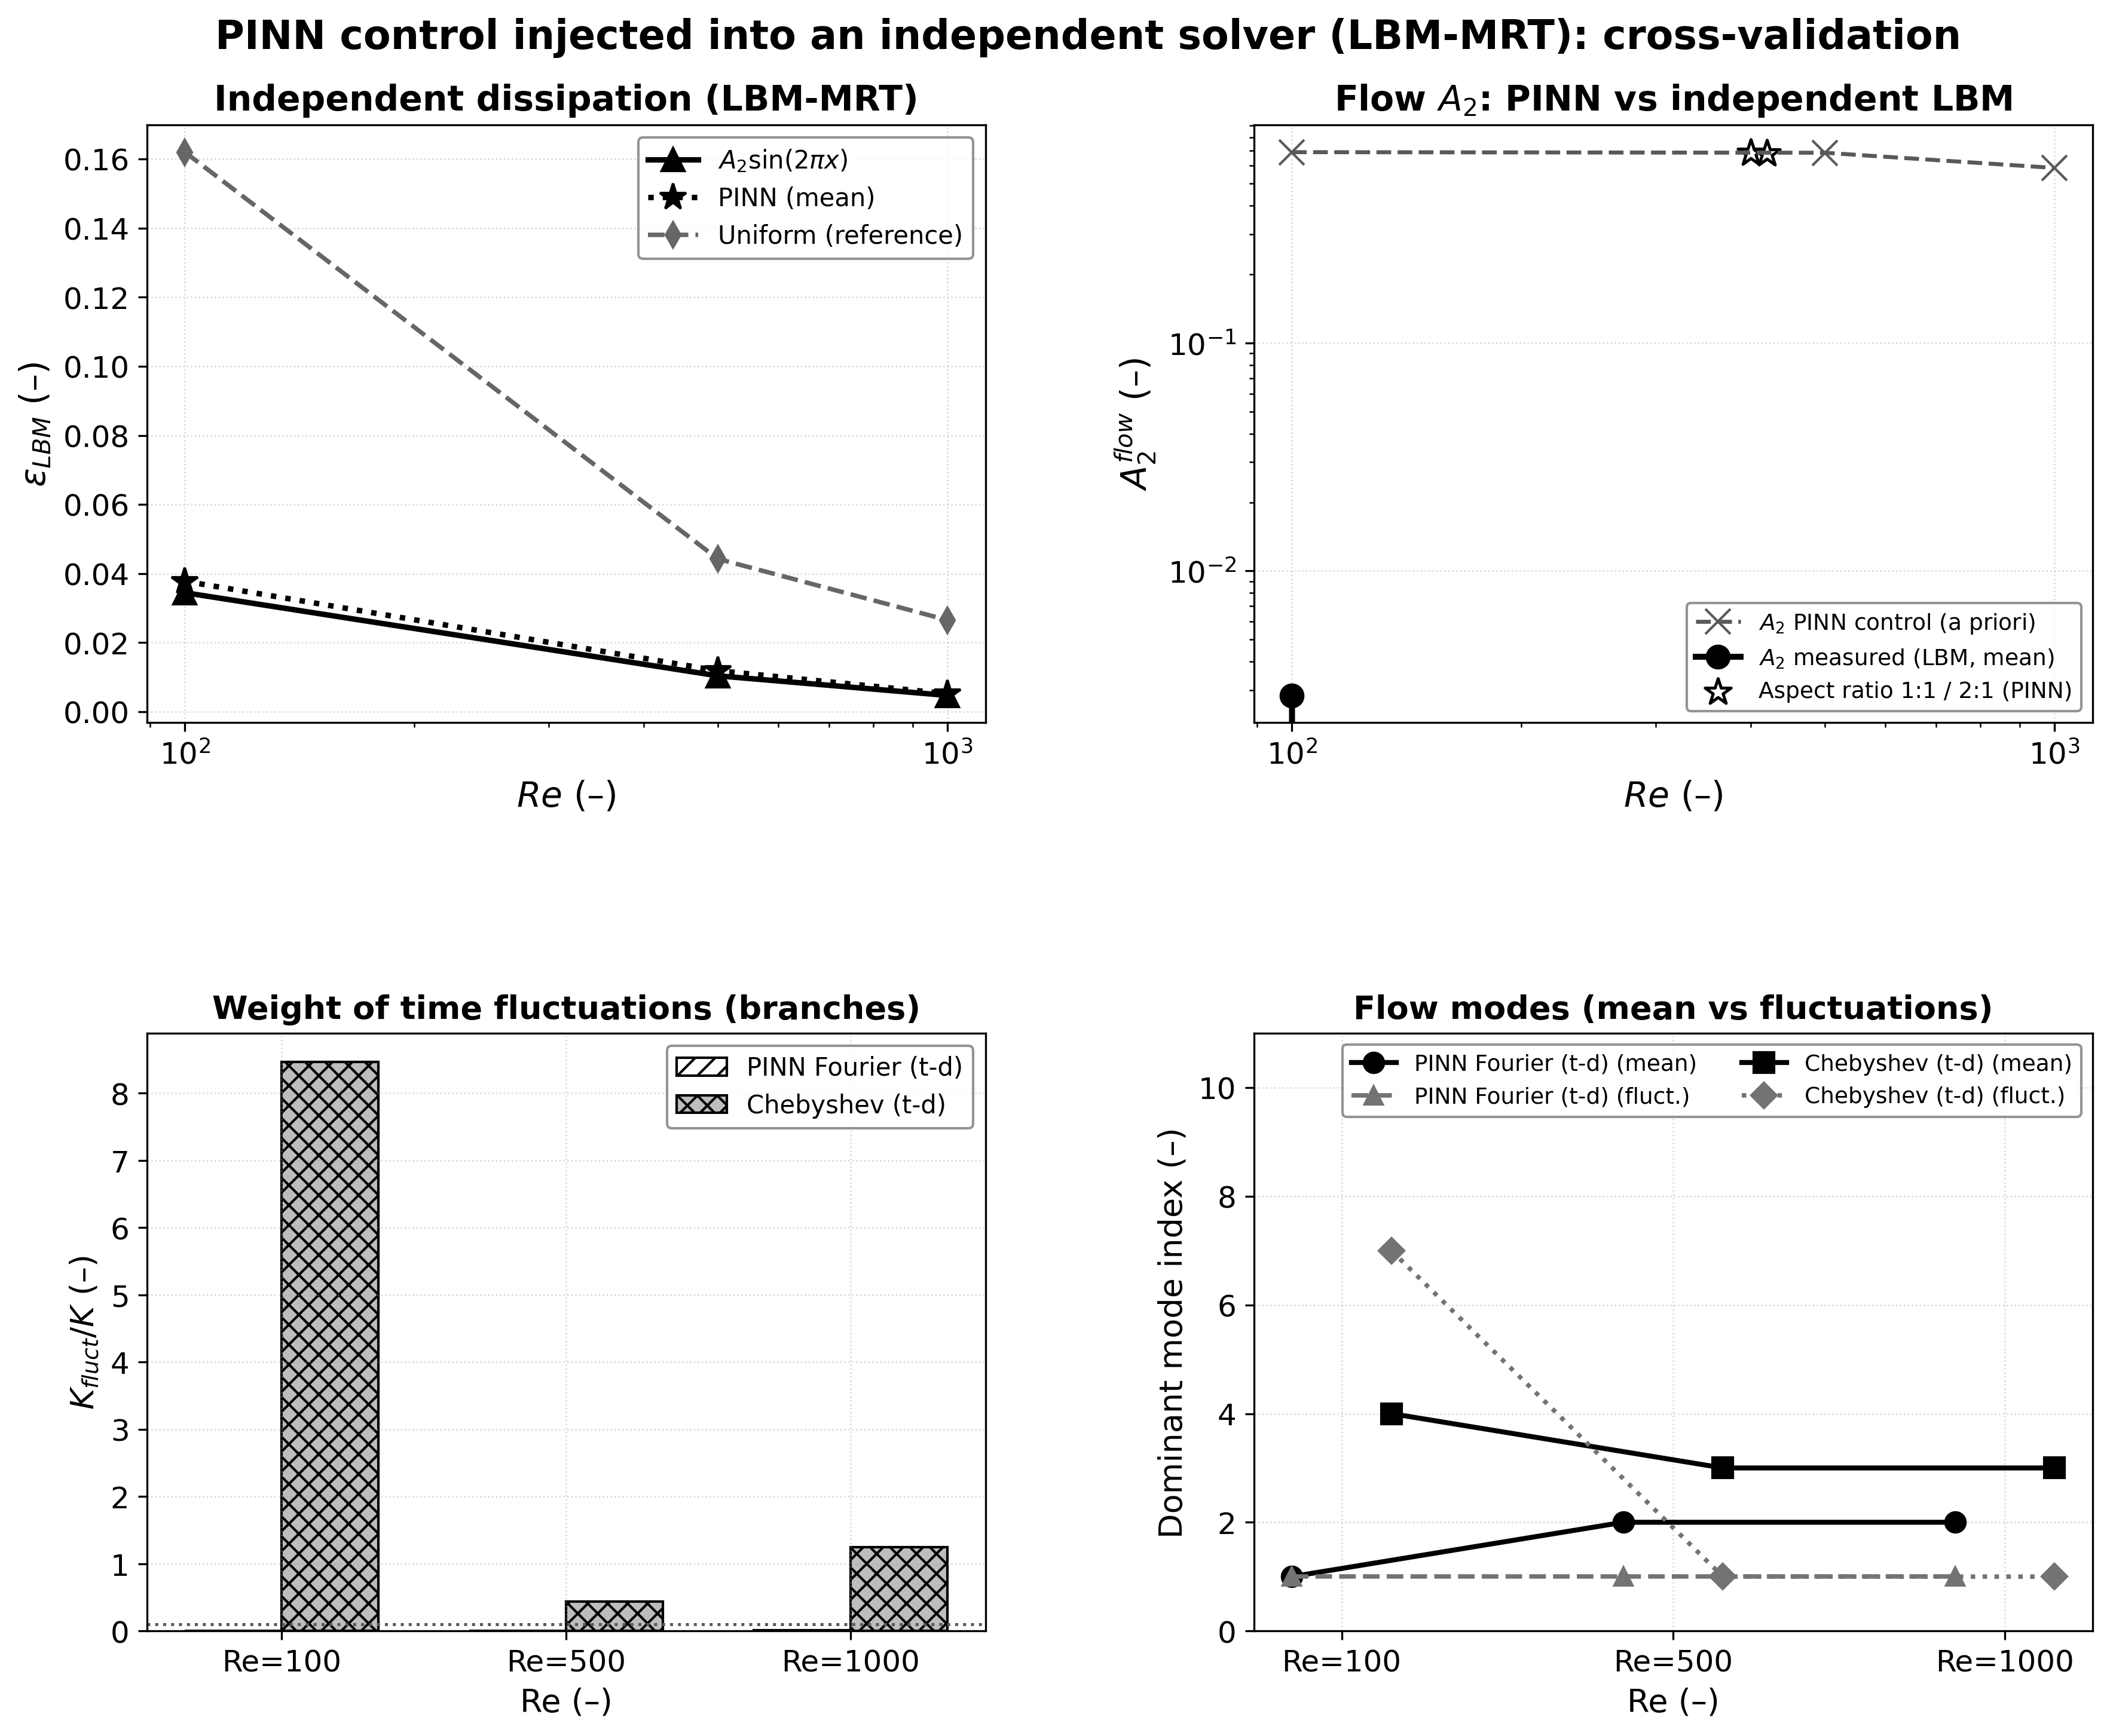
\includegraphics[width=\linewidth]{figures/fig12_consolidated.png}
\caption{\label{fig:consolidated} Consolidated comparison between the PINN identification and the independent LBM realization. (a) Integrated dissipation of the realized flows under the $A_2\sin(2\pi x)$ control, the complete PINN control, and the uniform reference, versus $\re$. (b) Second-mode amplitude: the PINN control coefficient $a_2^{\mathrm{ctrl}}$ (dashed) and the flow amplitude $a_2^{\mathrm{flow}}$ extracted from the vertical centerline $u(0.5,y)$ of the LBM mean field (solid), together with the square and $2{:}1$ aspect-ratio values. (c) Fluctuating-to-mean-flow kinetic ratio $R_K=K_{\mathrm{fluct}}/K_{\mathrm{mean}}$ for the Fourier and Chebyshev time-dependent branches, with the adopted $1\%$ admissibility threshold (dotted). (d) Dominant mode index of the mean field and of the fluctuations for the two branches. The Fourier branch passes the admissibility test; the Chebyshev branch fails it.}
\end{figure*}

\section{Symbolic regression of the identified control}\label{sec:sr}

As a complementary interpretability step, the sampled identified control field is submitted to symbolic regression (PySR \cite{cranmer2023pysr}) over a prescribed dictionary of elementary algebraic and trigonometric operators. Symbolic regression \emph{summarizes} the identified Fourier branch in a compact form; it does not constitute an independent optimization or physical-validation procedure, and its output is not used as evidence of optimality. Applied to the sampled control field, the regression converges to compact expressions dominated by a single trigonometric function of the spatial coordinate, of the generic form
\begin{equation}\label{eq:sr}
U_{\mathrm{SR}}\simeq a\left[b+\cos(\omega x-\varphi)\right]^{2}\left(c_{0}+c_{1}x+c_{2}t+c_{3}\re\right)+c_{4},
\end{equation}
with a fitted angular frequency $\omega\simeq3.42$ and a slowly varying linear envelope. The oscillatory kernel, together with the nearly Reynolds-independent envelope, reproduces the second-mode-dominated content of the identified Fourier branch; the temporal content of that branch is weak in the identified control (Table~\ref{tab:baseline}), and this should not be confused with the quasi-stationary character of the realized flow under the LBM verification (Section~\ref{sec:stationarity}). The generalization of the symbolic representation is assessed by a leave-one-condition-out (LOCO) procedure, in which the regression is trained on all Reynolds conditions except one and evaluated on the excluded one; the resulting coefficients of determination are reported in Table~\ref{tab:loco}. The high values indicate that the compact symbolic representation generalizes well across the tested range, consistent with the modal analysis of Section~\ref{sec:param}: the second spatial harmonic dominates the identified control, and the symbolic expressions combine it with a weak envelope rather than isolating a single factorized mode. The retained coefficients vary between fits, so the symbolic laws are best regarded as compact interpretive summaries rather than canonical expressions; they are retained only for the tested range and do not extrapolate.

\begin{table}[t]
\caption{\label{tab:loco} Leave-one-condition-out evaluation of the symbolic representation. $R^2$ is the coefficient of determination of the expression trained on all conditions except the indicated one, evaluated on the excluded condition.}
\centering
\begin{tabular}{cccccccccc}
\toprule
$\re_{\mathrm{held-out}}$ & 100 & 300 & 400 & 500 & 600 & 700 & 800 & 900 & 1000 \\
\midrule
$R^2$ & 0.9885 & 0.9666 & 0.9685 & 0.9908 & 0.9748 & 0.9595 & 0.9500 & 0.9326 & 0.9820 \\
\bottomrule
\end{tabular}
\end{table}

\section{Discussion}\label{sec:discussion}

\subsection{What the term \emph{modal collapse} does and does not claim}

The modal analysis establishes that the identified control concentrates its energy in one stationary spatial mode, and we refer to this concentration as a conditional modal collapse. The qualifier is essential: the collapse is recovered for the tested parametrizations, targets, seeds, capacities, and aspect ratios, but it is not a universal property of the lid-driven-cavity control problem. In particular: (i) it is basis-dependent, as the modified-Chebyshev parametrization produces a temporally dominated branch; (ii) it is initialization-dependent, as a subset of random initializations reaches a temporal branch of comparable objective; and (iii) its regime is limited in Reynolds number and actuation energy, as documented at $\re=1000$ and $E^*\ge0.5$. We therefore read the modal collapse as a structure of the identification problem rather than a physical law of the flow.

\subsection{Comparison with reduced-order and physics-informed literature}

Reduced-order analyses of the lid-driven cavity and of related benchmark flows identify the dominant spatial modes of the flow, and control efforts built on these modes are known to be robust within their validity range \cite{rowley2004model,noack2003hierarchy,taira2017modal}. Our result is consistent with this picture at the level of the realized flow: the second-mode hypothesis is reproduced by an independent solver as a low-dissipation, quasi-stationary branch \cite{ghia1982high}. However, our analysis differs from the classical reduced-order workflow in that the dominant structure is identified by optimizing the \emph{control} against a physics-informed loss, not by extracting the flow modes from snapshots; the two objects (control coefficient $a_2^{\mathrm{ctrl}}$ and flow response $a_2^{\mathrm{flow}}$) are related but distinct, and both are verified independently. The parametrization sensitivity we observe echoes known results on the non-uniqueness of data-driven representations \cite{brunton2015closed,taira2017modal}: different bases give different, equally well-trained controls, and only the independent verification discriminates them. Physics-informed optimization has also been reported to be sensitive to the loss composition and to the network initialization \cite{raissi2019physics,karniadakis2021physics,cuomo2022}, in line with our seed and ablation results.

\subsection{Limitations}

The study is deliberately bounded. First, the verification is numerical and limited to the two-dimensional lid-driven cavity, to the tested Reynolds range, and to the realized operating points; no claim of physical optimality is made for the recovered branch. Second, the operational quasi-stationarity criterion ($R_K<1\%$) is a threshold, not a proof of stationarity; it is adapted to the advection time scale used here and may be re-posed for other flows. Third, the GCI is established for the dissipation metric on one control; the $11\%$ uncertainty at the production resolution bounds, but does not eliminate, the discretization effect on the smaller reported differences. Fourth, the symbolic regression is a descriptive fit, retained for interpretability only.

\section{Conclusions}\label{sec:conclusions}

We have used a parametric physics-informed neural network to identify a distributed lid actuation for the lid-driven cavity over $100\le\re\le1000$, and we have characterized the structure of the identified control through systematic robustness, parametrization, and independent-verification campaigns. Within the Fourier parameterization, the identification recovers, across the tested actuation energies, network capacities, basis sizes, and aspect ratios, a branch dominated by a single stationary second spatial mode, which concentrates more than $91\%$ of the control energy at $\re=100$ and $500$. This branch: (i) is robust to moderate changes of the actuation-energy target, the cavity aspect ratio, and the network architecture and basis size, within the tested ranges; (ii) is strongly influenced in its branch selection by the variance regularization, as demonstrated by loss ablation; (iii) is reproduced by an independent LBM solver as a low-dissipation, quasi-stationary flow whose fluctuating kinetic energy remains below $1\%$ of the mean-flow kinetic energy; and (iv) is not universal, because at $\re=1000$ the modal concentration weakens, because a subset of random initializations reaches a temporal branch of comparable objective, and because a modified-Chebyshev parametrization produces a temporally dominated branch that fails the adopted LBM admissibility test. We conclude that the second-mode-dominated control is a repeatedly recoverable, \emph{parameterization-conditioned} branch of the identification problem rather than a universal optimum, and we recommend that physics-informed control identification be accompanied by systematic branch analysis and independent numerical verification before a recovered control is interpreted physically. Methodologically, the study demonstrates that branch characterization combined with independent numerical verification can discriminate a branch that is reproduced across methods from a parametrization-contingent alternative, which we regard as the main methodological contribution of the work.

\begin{acknowledgments}
This work benefited from the reviewers' comments, which motivated the independent LBM verification and the systematic branch-analysis and parametrization campaigns. The data and codes supporting the reported results are available in the public repository cited in the Data and code availability section.
\end{acknowledgments}

\section*{Data and code availability}
% AIP request: data and software availability statements plus dataset citation in the bibliography.
The data (CSV tables) and codes (PINN and LBM) supporting this article are available in the public repository cited as Ref.~\onlinecite{repo2026}; see also the Supplementary Material.

\begin{thebibliography}{99}

\bibitem{repo2026}
A. Beniaiche, ``PINN identification and LBM validation of lid-driven-cavity control,'' public repository, https://github.com/geminiahmed25-Ahkat/pinn-lid-driven-cavity (2026).

\bibitem{brunton2015closed} S. L. Brunton and B. R. Noack, ``Closed-loop turbulence control: Progress and challenges,'' Appl. Mech. Rev. \textbf{67}, 050801 (2015).

\bibitem{gad2000flow} M. Gad-el-Hak, \emph{Flow Control: Passive, Active, and Reactive Flow Management} (Cambridge University Press, Cambridge, 2000).

\bibitem{ghia1982high} U. Ghia, K. N. Ghia, and C. T. Shin, ``High-Re solutions for incompressible flow using the Navier--Stokes equations and a multigrid method,'' J. Comput. Phys. \textbf{48}, 387--411 (1982).

\bibitem{bewley2001dns} T. R. Bewley, P. Moin, and R. Temam, ``DNS-based predictive control of turbulence: an optimal benchmark for feedback algorithms,'' J. Fluid Mech. \textbf{447}, 179--225 (2001).

\bibitem{rowley2004model} C. W. Rowley, T. Colonius, and R. M. Murray, ``Model reduction for compressible flows using POD and Galerkin projection,'' Physica D \textbf{189}, 115--129 (2004).

\bibitem{bergmann2005optimal} M. Bergmann, L. Cordier, and J.-P. Brancher, ``Optimal rotary control of the cylinder wake using proper orthogonal decomposition reduced-order model,'' Phys. Fluids \textbf{17}, 097101 (2005).

\bibitem{noack2003hierarchy} B. R. Noack, K. Afanasiev, M. Morzy\'nski, G. Tadmor, and F. Thiele, ``A hierarchy of low-dimensional models for the transient and post-transient cylinder wake,'' J. Fluid Mech. \textbf{497}, 335--363 (2003).

\bibitem{taira2017modal} K. Taira, S. L. Brunton, S. T. M. Dawson, C. W. Rowley, T. Colonius, B. J. McKeon, O. T. Schmidt, S. Gordeyev, V. Theofilis, and L. S. Ukeiley, ``Modal analysis of fluid flows: An overview,'' AIAA J. \textbf{55}, 4013--4041 (2017).

\bibitem{raissi2019physics} M. Raissi, P. Perdikaris, and G. E. Karniadakis, ``Physics-informed neural networks: A deep learning framework for solving forward and inverse problems involving nonlinear partial differential equations,'' J. Comput. Phys. \textbf{378}, 686--707 (2019).

\bibitem{karniadakis2021physics} G. E. Karniadakis, I. G. Kevrekidis, L. Lu, P. Perdikaris, S. Wang, and L. Yang, ``Physics-informed machine learning,'' Nat. Rev. Phys. \textbf{3}, 422--440 (2021).

\bibitem{raissi2020hidden} M. Raissi, A. Yazdani, and G. E. Karniadakis, ``Hidden fluid mechanics: Learning velocity and pressure fields from flow visualizations,'' Science \textbf{367}, 1026--1030 (2020).

\bibitem{jin2021nsfnets} X. Jin, S. Cai, H. Li, and G. E. Karniadakis, ``NSFnets (Navier--Stokes flow nets): Physics-informed neural networks for the incompressible Navier--Stokes equations,'' J. Comput. Phys. \textbf{426}, 109951 (2021).

\bibitem{sun2020surrogate} L. Sun, H. Gao, S. Pan, and J.-X. Wang, ``Surrogate modeling for fluid flows based on physics-constrained deep learning without simulation data,'' Comput. Methods Appl. Mech. Eng. \textbf{361}, 112732 (2020).

\bibitem{cuomo2022} S. Cuomo, V. S. Di Cola, F. Giampaolo, G. Rozza, M. Raissi, and F. Piccialli, ``Scientific machine learning through physics-informed neural networks: Where we are and what is next,'' J. Sci. Comput. \textbf{92}, 88 (2022).

\bibitem{velivelli2024pinn} A. Velivelli et al., ``Physics-informed neural network for the inverse identification of boundary conditions and model parameters,'' Phys. Fluids \textbf{36}, 023332 (2024).

\bibitem{kingma2015adam} D. P. Kingma and J. Ba, ``Adam: A method for stochastic optimization,'' in \emph{Proceedings of the 3rd International Conference on Learning Representations (ICLR)}, San Diego (2015).

\bibitem{succi2001lattice} S. Succi, \emph{The Lattice Boltzmann Equation for Fluid Dynamics and Beyond} (Oxford University Press, Oxford, 2001).

\bibitem{cranmer2023pysr} M. Cranmer et al., ``Interpretable machine learning for science with PySR and SymbolicRegression.jl,'' arXiv:2305.01582 (2023).

\end{thebibliography}

\end{document}